\documentclass[10pt]{article}

\usepackage[top=0.80in, bottom=0.80in, left=0.80in, right=0.80in]{geometry}
\usepackage{amsmath, amssymb, amsfonts, mathtools}
\usepackage{graphicx}
\usepackage[table]{xcolor}
\usepackage[hyphens]{url}
\usepackage[hidelinks,colorlinks=true,linkcolor=blue!70!black,citecolor=blue!70!black,urlcolor=blue!70!black]{hyperref}
\usepackage{booktabs}
\usepackage{tabularx}
\usepackage{longtable}
\usepackage{array}
\usepackage{multirow}
\usepackage{caption}
\usepackage{fancyhdr}
\usepackage{listings}
\usepackage{cite}
\usepackage{microtype}
\usepackage{enumitem}

% Float placement parameters
\renewcommand{\topfraction}{0.95}
\renewcommand{\bottomfraction}{0.95}
\renewcommand{\textfraction}{0.05}
\renewcommand{\floatpagefraction}{0.85}

% Header and Footer configuration
\pagestyle{fancy}
\fancyhf{}
\rhead{\small QuietBox 2 Circulant DMA AR4JA LDPC Decoder Architecture \& DSN TDM Operations}
\lhead{\small Technical Monograph}
\rfoot{\small Page \thepage}
\lfoot{\footnotesize Dr. Christopher R. Jones --- Tenstorrent QuietBox 2 / CCSDS AR4JA LDPC Research}
\renewcommand{\headrulewidth}{0.6pt}
\renewcommand{\footrulewidth}{0.4pt}

% Custom colors
\definecolor{boxbg}{RGB}{244, 247, 252}
\definecolor{boxframe}{RGB}{31, 97, 141}
\definecolor{warnbg}{RGB}{253, 246, 238}
\definecolor{warnframe}{RGB}{192, 80, 30}
\definecolor{codebg}{RGB}{245, 247, 250}
\definecolor{codegreen}{RGB}{28, 128, 64}
\definecolor{codepurple}{RGB}{118, 42, 131}
\definecolor{codeblue}{RGB}{21, 76, 153}

\newcommand{\archBox}[2]{%
\vspace{0.5em}\noindent\fcolorbox{boxframe}{boxbg}{%
\parbox{0.975\textwidth}{%
\vspace{0.25em}\textbf{\textcolor{boxframe}{#1:}}\ #2\vspace{0.25em}
}}%
\vspace{0.6em}
}

\newcommand{\invariantBox}[2]{%
\vspace{0.5em}\noindent\fcolorbox{warnframe}{warnbg}{%
\parbox{0.975\textwidth}{%
\vspace{0.25em}\textbf{\textcolor{warnframe}{#1:}}\ #2\vspace{0.25em}
}}%
\vspace{0.6em}
}

\lstdefinestyle{ttcpp}{
    backgroundcolor=\color{codebg},
    commentstyle=\color{codegreen}\itshape,
    keywordstyle=\color{codeblue}\bfseries,
    numberstyle=\tiny\color{gray},
    stringstyle=\color{codepurple},
    basicstyle=\ttfamily\footnotesize,
    breakatwhitespace=false,
    breaklines=true,
    captionpos=b,
    keepspaces=true,
    numbers=left,
    numbersep=6pt,
    showspaces=false,
    showstringspaces=false,
    showtabs=false,
    tabsize=2,
    frame=single,
    rulecolor=\color{gray!40}
}
\lstset{style=ttcpp}

\newcolumntype{L}[1]{>{\raggedright\arraybackslash}p{#1}}
\newcolumntype{C}[1]{>{\centering\arraybackslash}p{#1}}
\newcolumntype{R}[1]{>{\raggedleft\arraybackslash}p{#1}}

\title{\textbf{\LARGE Ultra-High-Throughput Quasi-Cyclic LDPC Decoding on the Tenstorrent QuietBox 2:}\\[0.35em]
\Large Complete Microarchitectural Specification, 5.485 Gsps Circulant DMA Engine, 40-Billion-Block Deep Error-Floor Certification, and Global NASA Deep Space Network (DSN) Time-Division Multiplexing}

\author{%
\textbf{Dr. Christopher R. Jones}\\[0.35em]
\small JPL Staff Alumni%
}
\date{November 2026}

\begin{document}

\maketitle

\begin{abstract}
This monograph presents the complete architectural, mathematical, microarchitectural, and operational specification of the production \textbf{Circulant DMA 4-Codeword Low-Density Parity-Check (LDPC) Decoder and Monte Carlo Simulation Engine} deployed on the \textbf{Tenstorrent QuietBox~2 (QB2)} desktop supercomputing workstation. Targeting the Consultative Committee for Space Data Systems (CCSDS) 131.0-B-5 Accumulate-Repeat-4-Jagged-Accumulate (AR4JA) Rate-1/2 code ($N=2560$ variable nodes, $K=1024$ information bits, $M=1536$ parity checks, punctured by $P=512$ nodes to $N_{\mathrm{tx}}=2048$ transmitted channel symbols with quasi-cyclic lifting factor $Z=128$), the engine harnesses all \textbf{440 Blackhole Tensix compute cores} (2,200 RISC-V processors and 440 32-lane Vector SFPU engines) across four liquid-cooled Blackhole ASICs in a $2 \times 2$ mesh.

By exploiting the quasi-cyclic contiguity invariant $\Delta v / \Delta c = +1$ of the AR4JA parity-check matrix, our architecture replaces legacy scalar pointer-chasing ($\sim 3,300\ \mathrm{cycles/tile}$) with stateful 512-bit (64-byte/cycle) L1 Network-on-Chip (NoC) Direct Memory Access (DMA) slice bursts requiring only \textbf{2 clock cycles per 128-byte 4-codeword transfer}. Coupled with an in-place row-layered Gauss-Seidel schedule, a zero-transpose 32-lane SIMD pairwise tree implementation of Dr.~C.~R.~Jones' true recursive \textbf{Approximate-Min*} algorithm (with dyadic intrinsic check-message damping $\beta = 0.9375 = 15/16$ and dual-tier IEEE Round-to-Nearest-Even \texttt{bfloat16} quantization), unconditional blind DMA scatter with immediate convergence latching, and a four-stage microarchitectural optimization campaign, exact hardware per-tile turnaround is compressed from $3,856.7\ \mathrm{cycles/tile}$ to $\mathbf{3,481.0\ \mathrm{cycles/tile}}$ ($-9.74\%$). Across the 440-core mesh, the engine achieves a sustained decoding throughput of $\mathbf{5,287.3\ \mathrm{Msps}}$ ($\mathbf{5.29\ \mathrm{Gsps}}$) at the default $1,350\ \mathrm{MHz}$ ASIC clock and $\mathbf{5,484.5\ \mathrm{Msps}}$ ($\mathbf{5.485\ \mathrm{Gsps}}$ raw symbol rate / $\mathbf{2.742\ \mathrm{Gbps}}$ information rate) at the $1,400\ \mathrm{MHz}$ ARC firmware ceiling---a $\mathbf{194.5\times}$ speedup over the single-worker scalar baseline ($28.2\ \mathrm{Msps}$) and a $\mathbf{31.8\times\text{--}33.0\times}$ speedup over the 5-worker dual-codeword packed scalar architecture ($166.4\text{--}173.9\ \mathrm{Msps}$).

At $5.485\ \mathrm{Gsps}$, a 10-billion-block ($20.48\ \mathrm{trillion}$ symbol) deep error-floor campaign executes in $\mathbf{62.2\ \mathrm{minutes}}$ ($3,734\ \mathrm{seconds}$). Across four independent 10-billion-block certification runs at $E_b/N_0 = 2.50\ \mathrm{dB}$ (\textbf{40 billion blocks / $81.92\ \mathrm{trillion}$ symbols total}), the engine recorded \textbf{61 Frame Errors} ($\mathrm{FER} = 1.525 \times 10^{-9}$, $95\%$ Poisson CI: $[1.17, 1.96] \times 10^{-9}$) and down to $\mathrm{FER} = 8.00 \times 10^{-10}$ (Circulant DMA) and $3.00 \times 10^{-10}$ (Scalar 5W) across 10 billion blocks at $2.60\ \mathrm{dB}$. In $100\%$ of observed failures, parity syndromes remained unsatisfied ($H\hat{\mathbf{c}}^T \ne \mathbf{0}$), proving that deep-floor events arise exclusively from graphical trapping sets rather than undetected minimum-distance codewords. Furthermore, because the unit-stride circulant contiguity law ($\Delta v / \Delta c = +1$) and $L \ge 32$ sub-circulant lifting hold universally across the standard, the architecture natively supports \textbf{all 9 CCSDS 131.0-B-5 AR4JA codes} ($K \in \{1024, 4096, 16384\}$, Rates $r \in \{1/2, 2/3, 4/5\}$) entirely within single-core $1,536\ \mathrm{KB}$ L1 SRAM, and introduces \textbf{circulant family descriptive compression} wherein each block-length family is canonically described by its \textbf{Rate-4/5 mother code} ($H_{1/2}$ and $H_{2/3}$ being exact right-justified column sub-matrices of $H_{4/5}$ with zero Frobenius difference). Finally, we present a complete system architecture showing how \textbf{a single $\$9,999$ QuietBox~2 workstation can simultaneously decode the entire planetary NASA Deep Space Network (DSN)} across all three global complexes (Goldstone, Madrid, and Canberra) via Time-Division Multiplexing (TDM) while utilizing less than $22\%$ of its sustained compute capacity.
\end{abstract}

\newpage
\tableofcontents
\newpage

% ==============================================================================
\section{Executive Summary and Architectural Paradigm Shift}
\label{sec:exec_summary}
% ==============================================================================

Deep-space telemetry and high-reliability satellite communications demand Forward Error Correction (FEC) codes capable of operating within fractions of a decibel of the Shannon limit while guaranteeing ultra-low Frame Error Rates ($\mathrm{FER} \le 10^{-8}$ to $10^{-10}$) without catastrophic error floors. The Consultative Committee for Space Data Systems (CCSDS) Accumulate-Repeat-4-Jagged-Accumulate (AR4JA) Low-Density Parity-Check (LDPC) code family \cite{ccsds_tm_coding, divsalar_linear_distance, andrews_deep_space_ldpc} was engineered to satisfy both requirements by combining protograph linear minimum-distance growth with quasi-cyclic (QC) hardware routability.

Historically, empirically certifying LDPC decoder behavior in the $10^{-9}$ to $10^{-10}$ FER regime has been a formidable computational barrier. Resolving a single SNR point at $\mathrm{FER} \approx 10^{-9}$ with statistical confidence requires simulating $10^{10}$ to $4 \times 10^{10}$ codewords ($2.05 \times 10^{13}$ to $8.19 \times 10^{13}$ channel symbols). On conventional multi-core CPU clusters or legacy FPGA testbeds, such a campaign requires weeks of wall-clock execution per operating point, rendering systematic parametric studies of quantization, message damping, schedule ordering, and trapping-set rescue algorithms impractical.

This monograph documents a fundamental paradigm shift in high-throughput iterative decoding and Monte Carlo error-floor investigation: mapping both the Additive White Gaussian Noise (AWGN) channel synthesis and the iterative belief-propagation decoder entirely inside the distributed on-die L1 SRAM and 32-lane Single-Instruction Multiple-Data (SIMD) Special Function Processing Units (SFPUs) of a commercial off-the-shelf (COTS) parallel AI/ML inference workstation---the \textbf{Tenstorrent QuietBox~2 (QB2)}.

\subsection{Summary of Key Technical Achievements}

\begin{enumerate}[leftmargin=1.8em, itemsep=3pt]
    \item \textbf{Multi-Gigabit Sustained Silicon Throughput ($5.29\text{--}5.485\ \mathrm{Gsps}$)}: The flagship \textbf{Circulant DMA 4-Codeword Engine} (\texttt{engines/circulant\_dma\_4cw/}) sustains $\mathbf{5,287.3\ \mathrm{Msps}}$ ($\mathbf{5.29\ \mathrm{Gsps}}$) at the default $1,350\ \mathrm{MHz}$ Blackhole ASIC clock and $\mathbf{5,484.5\ \mathrm{Msps}}$ ($\mathbf{5.485\ \mathrm{Gsps}}$ channel symbol rate / $\mathbf{2.742\ \mathrm{Gbps}}$ information bit rate) when locked to the $1,400\ \mathrm{MHz}$ ARC firmware ceiling across all 440 Tensix cores during full 200-iteration maximum-ceiling Monte Carlo sweeps. This represents a $\mathbf{194.5\times}$ speedup over the single-TRISC scalar baseline ($28.2\ \mathrm{Msps}$) and a $\mathbf{31.8\times\text{--}33.0\times}$ speedup over the 5-worker dual-codeword packed scalar engine ($166.4\text{--}173.9\ \mathrm{Msps}$).
    \item \textbf{Elimination of the 3,300-Cycle Gather/Scatter Memory Bottleneck}: By exploiting the quasi-cyclic circulant contiguity law ($\Delta v / \Delta c = +1$) of the CCSDS AR4JA matrix (\texttt{makeH\_AR4JA.m}), consecutive check rows address contiguous variable nodes in L1 SRAM. Packing 4 codewords per variable node (\texttt{Packed4CW\_BF16}, $8\ \mathrm{bytes/node}$) transforms each 16-check face edge into a contiguous $128\text{-byte}$ slice transferred by the Blackhole $512\text{-bit}$ ($64\ \mathrm{B/cycle}$) L1 Network-on-Chip (NoC) DMA engine in \textbf{2 clock cycles}, reducing gather and scatter latencies from $\sim 3,300\ \mathrm{cycles/tile}$ to $\mathbf{636.0\ \mathrm{cycles/tile}}$ and $\mathbf{744.0\ \mathrm{cycles/tile}}$, respectively.
    \item \textbf{Zero-Transpose 32-Lane SFPU Pairwise $\mathrm{AMin}^*$ Tree with Intrinsic Damping ($\beta = 15/16$)}: On the Tensix 32-lane SFPU, the native hardware subvector transpose instruction (\texttt{SFPTRANSP} / \texttt{swap\_subvec16}) destructively clobbers vector registers $L_4 \dots L_7$. We eliminate $100\%$ of \texttt{SFPTRANSP} operations by organizing tile faces so that check edges $0 \dots 2$ occupy Faces $0$ and $1$ (\texttt{dst\_reg[0..15]}) while edges $3 \dots 5$ occupy Faces $2$ and $3$ (\texttt{dst\_reg[16..31]}). Worker~3 (\texttt{TRISC1}) fuses single-load sign-parity XOR accumulation with pairwise reductions $M_{03}, M_{14}, M_{25}$ staged in unused face registers \texttt{6..7}, applies Dr.~Jones' 2-region piecewise linear Approximate-Min* correction \cite{jones_approx_min_star}, scales outgoing check magnitudes by the exact dyadic damping factor $\beta = 0.9375 = 15/16$, and applies dual-tier IEEE Round-to-Nearest-Even (\texttt{round\_bf16} vs.\ \texttt{round\_bf16\_fast}) in $\mathbf{1,764.5\ \mathrm{cycles/tile}}$.
    \item \textbf{4-Stage Microarchitectural Cycle Compression ($3,856.7 \to 3,481.0\ \mathrm{cyc/tile}$)}: Gapless hardware wall-clock cycle telemetry (\texttt{T0} through \texttt{T5} on Core \texttt{(0,0)}) guided four targeted optimizations---stateful one-packet NoC DMA with inline 8-byte wrap copies ($-86.4\ \mathrm{cyc/tile}$), fused SFPU sign/pairwise loads with mask-free \texttt{round\_bf16\_fast} on direct 16-bit \texttt{dst\_reg} stores ($-110.8\ \mathrm{cyc/tile}$), decoupled Tile~39 \texttt{BRISC} parity scanning overlapping \texttt{NCRISC} teardown ($-180.8\ \mathrm{cyc/tile}$), and complete compile-time elimination of RISC-V \texttt{divu}/\texttt{remu} instructions---reducing exact tile turnaround by $\mathbf{-375.7\ \mathrm{cycles/tile}}$ ($\mathbf{-9.74\%}$).
    \item \textbf{40-Billion-Block ($81.92\ \mathrm{Trillion}$ Symbols) Statistical Certification at $2.50\ \mathrm{dB}$}: Executing 10 billion blocks in $\mathbf{62.2\ \mathrm{minutes}}$ ($1,400\ \mathrm{MHz}$) enabled four independent 10-billion-block certification runs at $E_b/N_0 = 2.50\ \mathrm{dB}$, recording $18, 12, 15,$ and $16$ frame errors (\textbf{61 total Frame Errors}, $8,548$ Bit Errors across $40,000,004,320$ blocks), establishing a ground-truth $\mathrm{FER} = \mathbf{1.525 \times 10^{-9}}$ ($95\%$ CI: $[1.17, 1.96] \times 10^{-9}$) and extending down to $\mathrm{FER} = \mathbf{8.00 \times 10^{-10}}$ (Circulant DMA) and $\mathbf{3.00 \times 10^{-10}}$ (Scalar 5W) across 10 billion blocks at $2.60\ \mathrm{dB}$.
    \item \textbf{Universal Support for All 9 CCSDS AR4JA Codes \& Rate-4/5 Mother-Code Descriptive Compression}: Triple-redundant mathematical and empirical validation (\texttt{tools/validate\_all\_9\_ar4ja\_codes.m}) proves that all 9 CCSDS 131.0-B-5 AR4JA codes ($K \in \{1024, 4096, 16384\}$, Rates $r \in \{1/2, 2/3, 4/5\}$) obey the unit-stride circulant contiguity invariant ($\Delta v / \Delta c = +1$) and fit 100\% inside single-core L1 SRAM ($2.2\%$ to $87.3\%$ decoder state). Moreover, for any submatrix size $M$, the lower-rate parity-check matrices $H_{1/2}(M)$ and $H_{2/3}(M)$ are exact right-justified column sub-matrices of the Rate-4/5 mother code $H_{4/5}(M)$ ($\| H_{\mathrm{sub}} - H_{4/5}[:, \mathrm{cols}] \|_F \equiv 0$), allowing each block-length family to be completely described by a single master Rate-4/5 circulant descriptor table with zero-cycle runtime rate switching.
    \item \textbf{Planetary-Scale NASA Deep Space Network (DSN) Consolidation via TDM}: We prove quantitatively that the aggregate telemetry downlink rate of the \emph{entire global NASA Deep Space Network} across Goldstone, Madrid, and Canberra ($\sim 35\text{--}40$ active spacecraft, $\approx 400\text{--}600\ \mathrm{Mbps}$ aggregate information rate) represents less than $\mathbf{22\%}$ of a single QuietBox~2's sustained decoding capacity, enabling a single $\$9,999$ liquid-cooled workstation to serve as a universal Time-Division Multiplexed (TDM) multi-mission DSN telemetry decoder with sub-millisecond frame latency.
\end{enumerate}

% ==============================================================================
\section{The Tenstorrent QuietBox 2 Platform: Hardware Architecture, Telemetry, and SWaP-C Economics}
\label{sec:qb2_hardware}
% ==============================================================================

A central engineering motivation of this work is demonstrating that modern spatially distributed AI inference accelerators---designed around dense arrays of SRAM-coupled RISC-V/SIMD cores connected by high-radix Networks-on-Chip (NoC)---map naturally to sparse graph message-passing algorithms that traditionally struggled on cache-coherent CPUs or warp-divergent GPUs.

\subsection{Workstation System Specifications and Physical Topology}

The Tenstorrent QuietBox~2 is a self-contained, whisper-quiet, closed-loop liquid-cooled desktop supercomputing workstation. Table~\ref{tab:qb2_specs} details the exact hardware and software configuration of our target production unit (\texttt{tt-quietbox}, IP \texttt{192.168.0.195}), verified directly via Linux kernel DMI tables, \texttt{lscpu}, \texttt{lspci}, and Tenstorrent System Management Interface (\texttt{tt-smi 6.8.0}) SMBus telemetry.

\begin{table}[!htbp]
\centering
\caption{\textbf{Tenstorrent QuietBox 2 Workstation Hardware, Firmware, and Cost Specifications.}}
\label{tab:qb2_specs}
\small
\begin{tabularx}{\textwidth}{@{}l L{4.6cm} X@{}}
\toprule
\textbf{Subsystem} & \textbf{Specification / Component} & \textbf{Architectural Details \& Measured Telemetry} \\
\midrule
\textbf{Workstation Model} & Tenstorrent QuietBox 2 (Blackhole Edition) & Commercial Off-The-Shelf (COTS) liquid-cooled desktop tower; retail acquisition cost $\mathbf{\$9,999\ \mathrm{USD}}$. \\
\addlinespace[3pt]
\textbf{Accelerator Cards} & $2 \times$ Tenstorrent Blackhole \texttt{p300c} Dual-ASIC PCIe Cards & Two dual-processor liquid-cooled PCIe Gen4 boards (\texttt{BOARD\_ID} \texttt{0x000004613193500a} and \texttt{0x0000046131935034}), housing \textbf{4 Blackhole ASICs} in a $2 \times 2$ mesh (\texttt{01:00.0} to \texttt{04:00.0}). \\
\addlinespace[3pt]
\textbf{Tensix Compute Grid} & $11 \times 10 = 110$ Tensix Cores / ASIC ($\mathbf{440\ \mathrm{Cores\ Total}}$) & Zero harvested compute rows (\texttt{HARVESTING\_STATE = 0x0} across all 4 chips); $\mathbf{2,200\ \mathrm{RISC\text{-}V\ Cores}}$ + $\mathbf{440\ \mathrm{Vector\ SFPUs}}$ ($14,080$ FP32/BF16 SIMD lanes). \\
\addlinespace[3pt]
\textbf{On-Die L1 SRAM} & $1.5\ \mathrm{MB}$ per Tensix Core ($\mathbf{660\ \mathrm{MB\ Aggregate\ L1}}$) & $165\ \mathrm{MB}$ L1 SRAM per Blackhole ASIC; tightly coupled to local NoC routers ($64\ \mathrm{B/cycle}$ per direction) with $>880\ \mathrm{TB/s}$ aggregate internal L1 bandwidth. \\
\addlinespace[3pt]
\textbf{Off-Chip DRAM} & $32\ \mathrm{GB}$ GDDR6 per ASIC ($\mathbf{128\ \mathrm{GB\ Total\ GDDR6}}$) & $8 \times 16\ \mathrm{Gbps}$ GDDR6 channels per ASIC (\texttt{enabled\_mask = 0xff}, $512\ \mathrm{GB/s}$ per ASIC, $2.05\ \mathrm{TB/s}$ aggregate DRAM bandwidth). \\
\addlinespace[3pt]
\textbf{ASIC Clock Domains} & \texttt{AICLK}: $1,350\ \mathrm{MHz}$ (Default) / $\mathbf{1,400\ \mathrm{MHz}}$ (\texttt{FORCE\_AICLK}) & Dynamic DVFS range $800\text{--}1,350\ \mathrm{MHz}$; lockable to $1,400\ \mathrm{MHz}$ ceiling via ARC msg \texttt{0x33}. \texttt{AXICLK}: $960\ \mathrm{MHz}$; \texttt{ARCCLK}: $800\ \mathrm{MHz}$. \\
\addlinespace[3pt]
\textbf{Thermal \& Power} & Closed-Loop Liquid Cooling ($\mathbf{47.5^\circ\mathrm{C}\text{--}51.2^\circ\mathrm{C}}$ Load) & Core voltage $0.81\text{--}0.82\ \mathrm{V}$; $\sim 263\text{--}266\ \mathrm{W}$ board power per dual-ASIC \texttt{p300c} card ($\mathbf{\sim 530\ \mathrm{W}}$ across all 4 ASICs; shutdown limit $110^\circ\mathrm{C}$). \\
\addlinespace[3pt]
\textbf{Host CPU \& Board} & AMD Ryzen 7 9700X (8C/16T Zen 5 @ $5.58\ \mathrm{GHz}$) & ASUS B850M-C AM5 micro-ATX motherboard; AVX-512 (\texttt{avx512\_bf16}, \texttt{avx512\_vnni}); PCIe Gen4 host fabric. \\
\addlinespace[3pt]
\textbf{Host System Memory} & $\mathbf{256\ \mathrm{GB}}$ DDR5 System RAM ($249.31\ \mathrm{GiB}$ Usable) & Supports massive host-side telemetry aggregation, multi-gigabyte matrix precomputation, and parallel compilation. \\
\addlinespace[3pt]
\textbf{OS \& Software Stack} & Ubuntu 24.04.4 LTS (Kernel \texttt{7.0.0-31-generic}) & TT-Metalium SDK \texttt{0.54}, Driver \texttt{TT-KMD 2.11.0}, \texttt{TT-UMD 0.9.12}, \texttt{pyluwen 0.10.0}, \texttt{riscv-tt-elf-g++} (SFPI \texttt{v7.89.0}). \\
\bottomrule
\end{tabularx}
\end{table}

\subsection{Internal Microarchitecture of a Single Blackhole Tensix Core}

Each of the 440 Tensix cores on the QuietBox~2 is a self-contained, heterogeneous dataflow processor integrating five independent 32-bit RISC-V instruction-issue pipelines, dedicated hardware DMA and data-transformation engines, and a $1,536\ \mathrm{KB}$ ($1.5\ \mathrm{MB}$) local L1 scratchpad SRAM:

\begin{enumerate}[leftmargin=1.8em, itemsep=2pt]
    \item \textbf{\texttt{BRISC} (Worker 0 --- RISC-V Data Movement Core 0)}: Controls Network-on-Chip Router~0 (\texttt{NOC\_0}), issuing asynchronous 512-bit ($64\ \mathrm{B/cycle}$) L1-to-L1 and DRAM-to-L1 DMA read/write packets. In our Circulant DMA engine, \texttt{BRISC} gathers and scatters check node edges for Checks $0 \dots 15$ (Faces $0$ and $2$) and executes the end-of-iteration information-bit parity scan.
    \item \textbf{\texttt{NCRISC} (Worker 1 --- RISC-V Data Movement Core 1)}: Controls Network-on-Chip Router~1 (\texttt{NOC\_1}), operating concurrently with \texttt{BRISC}. In our engine, \texttt{NCRISC} gathers and scatters check node edges for Checks $16 \dots 31$ (Faces $1$ and $3$), records gapless hardware wall-clock cycle timestamps (\texttt{T0..T5}) from physical register \texttt{0xFFB121F0}, and manages the syndrome convergence latch.
    \item \textbf{\texttt{TRISC0} (Worker 2 --- RISC-V Compute Unpack Thread)}: Programs and triggers the hardware \textbf{Unpacker Engine}, streaming $32 \times 32$ \texttt{bfloat16} tiles ($2,048\ \mathrm{bytes/tile}$) directly from L1 Circular Buffers (\texttt{CB\_SCRATCH\_GATHER} and \texttt{CB\_R\_MSG}) into the 64-register \texttt{DEST} register file in $126.5\ \mathrm{cycles/tile}$.
    \item \textbf{\texttt{TRISC1} (Worker 3 --- RISC-V Compute Math Thread)}: Drives the \textbf{32-Lane Vector Special Function Processing Unit (SFPU)} and Matrix Engine. Operating in native 16-bit \texttt{DEST} mode (\texttt{.fp32\_dest\_acc\_en = false}), \texttt{TRISC1} accesses all 64 \texttt{DEST} registers (\texttt{dst\_reg[0..63]}, each holding 32 lanes of 16-bit \texttt{bfloat16} data) and 8 transient 32-lane FP32 vector latches ($L_0 \dots L_7$), executing both the 32-lane \texttt{VectorXoshiro128Plus} Remez Box-Muller channel generator and the zero-transpose pairwise Approximate-Min* check-node kernel.
    \item \textbf{\texttt{TRISC2} (Worker 4 --- RISC-V Compute Pack Thread)}: Programs and triggers the hardware \textbf{Packer Engine}, streaming completed outgoing check messages $R_{\mathrm{new}}$ (\texttt{dst\_reg[0..31]}) to \texttt{CB\_R\_MSG} and updated variable-node posteriors $L_{\mathrm{new}}$ (\texttt{dst\_reg[32..63]}) to \texttt{CB\_SCRATCH\_SCATTER} in $209.9\ \mathrm{cycles/tile}$.
\end{enumerate}

\subsection{Capital Cost, Power, and Throughput Economics (SWaP-C Comparison)}

To appreciate the economic and operational impact of the QuietBox~2 implementation, Table~\ref{tab:swapc_comparison} compares our measured physical silicon performance against representative high-performance CPU clusters, enterprise data-center GPU servers, and custom FPGA ground-station decoders evaluating the same 200-iteration CCSDS AR4JA Rate-1/2 code.

\begin{table}[!htbp]
\centering
\caption{\textbf{Economic, Power, and Throughput Comparison Across Computing Platforms (AR4JA Rate-1/2, 200 Max Iterations).}}
\label{tab:swapc_comparison}
\resizebox{\textwidth}{!}{%
\begin{tabular}{@{}l r r r r r r@{}}
\toprule
\textbf{Platform / Architecture} & \textbf{Est. System Cost (USD)} & \textbf{Active Power (W)} & \textbf{Sustained Throughput} & \textbf{Energy Eff. (Msps/W)} & \textbf{Cost Eff. (Msps/\$1k)} & \textbf{Time for $10^{10}$ Blocks} \\
\midrule
64-Core Server CPU (AVX-512 OpenMP) & $\$12,000$ & $350\ \mathrm{W}$ & $\sim 45\ \mathrm{Msps}$ & $0.13$ & $3.75$ & $5.26\ \mathrm{days}$ \\
8-Node CPU Cluster (512 Cores Total) & $\$95,000$ & $2,800\ \mathrm{W}$ & $\sim 360\ \mathrm{Msps}$ & $0.13$ & $3.79$ & $15.8\ \mathrm{hours}$ \\
8$\times$ Data-Center GPU Server (H100/B200) & $\$250,000$ & $6,500\ \mathrm{W}$ & $\sim 3,200\ \mathrm{Msps}$ & $0.49$ & $12.80$ & $106.7\ \mathrm{min}$ \\
Custom Radiation/Ground FPGA Rack & $\$180,000$ & $800\ \mathrm{W}$ & $\sim 2,500\ \mathrm{Msps}$ & $3.13$ & $13.89$ & $136.5\ \mathrm{min}$ \\
\midrule
\textbf{QB2 Scalar 5-Worker Packed Engine} & $\mathbf{\$9,999}$ & $530\ \mathrm{W}$ & $173.9\ \mathrm{Msps}$ & $0.33$ & $17.39$ & $32.7\ \mathrm{hours}$ \\
\textbf{QB2 Circulant DMA ($1,350\ \mathrm{MHz}$ Default)} & $\mathbf{\$9,999}$ & $530\ \mathrm{W}$ & $\mathbf{5,287.3\ \mathrm{Msps}}$ & $\mathbf{9.98}$ & $\mathbf{528.8}$ & $\mathbf{64.6\ \mathrm{min}}$ \\
\textbf{QB2 Circulant DMA ($1,400\ \mathrm{MHz}$ Boost)} & $\mathbf{\$9,999}$ & $550\ \mathrm{W}$ & $\mathbf{5,484.5\ \mathrm{Msps}}$ & $\mathbf{9.97}$ & $\mathbf{548.5}$ & $\mathbf{62.2\ \mathrm{min}}$ \\
\bottomrule
\end{tabular}%
}
\end{table}

At $\mathbf{548.5\ \mathrm{Msps\ per\ \$1,000}}$ of capital cost and $\mathbf{\sim 10.0\ \mathrm{Msps/W}}$ of accelerator power, the QuietBox~2 Circulant DMA engine delivers an order-of-magnitude advantage in both capital efficiency ($>39\times$ vs.\ enterprise GPU/FPGA systems) and software agility (compiled in seconds from standard C++20/SFPI kernels rather than weeks of Verilog place-and-route).

% ==============================================================================
\section{CCSDS AR4JA Rate-1/2 Code Structure, Quasi-Cyclic Circulant Geometry, and Tile/Face Mapping}
\label{sec:code_structure}
% ==============================================================================

\subsection{Protograph Construction and Quasi-Cyclic Lifting ($Z = 128$)}

The CCSDS 131.0-B-5 AR4JA Rate-1/2 code ($K=1024$) \cite{ccsds_tm_coding} is constructed via a two-stage protograph expansion designed by Divsalar, Dolinar, Jones, and Andrews \cite{divsalar_linear_distance, andrews_deep_space_ldpc}:
\begin{itemize}[leftmargin=1.8em, itemsep=2pt]
    \item \textbf{Dimensions}: $N = 2,560$ total variable nodes, $M = 1,536$ parity-check constraints, and $K = N - M = 1,024$ information bits.
    \item \textbf{High-Degree Variable Node Puncturing}: The final $P = 512$ variable nodes ($v \in [2048, 2559]$) correspond to the accumulate-repeat state nodes of the protograph and are punctured prior to transmission ($L_v^{\mathrm{ch}} = 0.0$), yielding $N_{\mathrm{tx}} = N - P = 2,048$ transmitted channel symbols and an operational code rate of $R = K / N_{\mathrm{tx}} = 1024 / 2048 = 1/2$.
    \item \textbf{Block-Circulant Submatrix Structure}: The $1,536 \times 2,560$ parity-check matrix $H$ is partitioned into a $12 \times 20$ array of $Z \times Z$ submatrices where $Z = 128$. Each submatrix $H_{b_r, b_c}$ ($b_r \in \{0 \dots 11\}$, $b_c \in \{0 \dots 19\}$) is either a $128 \times 128$ all-zero matrix or a circulant permutation matrix $I_Z^{(\sigma)}$ obtained by cyclically right-shifting the $128 \times 128$ identity matrix by $\sigma \in \{0 \dots 127\}$ columns (or the superposition of two circulants in the repeat-accumulate columns, resolved into disjoint edge slots).
    \item \textbf{Exact Check-Node Degree Distribution}: Across all $M = 1,536$ check rows, exactly $512$ rows ($b_r \in \{0 \dots 3\}$, rows $0 \dots 511$) have check degree $d_c = 3$, and $1,024$ rows ($b_r \in \{4 \dots 11\}$, rows $512 \dots 1535$) have check degree $d_c = 6$. The total number of non-zero edges in the Tanner graph is:
    \begin{equation}
    E_{\mathrm{total}} = 512 \times 3 + 1,024 \times 6 = 1,536 + 6,144 = \mathbf{7,680\ \mathrm{edges}}.
    \end{equation}
\end{itemize}

\begin{figure}[!htbp]
\centering
\includegraphics[width=0.96\textwidth,height=0.72\textheight,keepaspectratio]{figures/ar4ja_h_matrix_tiles_and_faces_spy_plot.png}
\caption{\textbf{Master Structural Mapping of the CCSDS AR4JA Rate-1/2 Parity-Check Matrix ($1536 \times 2560$) onto the Tenstorrent Blackhole Tensix Architecture.} \textbf{(Panel A)} Full spy plot of the 7,680 non-zero edges partitioned into 40 row-layered scheduling tiles (8 Degree-3 tiles + 32 Degree-6 tiles). \textbf{(Panel B)} Tile degree distribution across the 40-tile schedule. \textbf{(Panel C)} Decomposition of each 32-check tile into four $16 \times 16$ hardware faces across Worker~0 (\texttt{BRISC}, Faces 0 \& 2) and Worker~1 (\texttt{NCRISC}, Faces 1 \& 3). \textbf{(Panel D)} Circulant contiguity ($\Delta v / \Delta c = +1$) enabling 2-cycle 128-byte (512-bit) L1 DMA slice bursts. \textbf{(Panel E)} Five RISC-V workers operating in lockstep with zero \texttt{SFPTRANSP} subvector transpositions. \textbf{(Panel F)} Spatial scaling across all 440 Tensix cores.}
\label{fig:spy_plot_master}
\end{figure}

\subsection{Breaking the 3,300-Cycle Memory Wall via the Circulant Contiguity Law ($\Delta v / \Delta c = +1$)}
\label{sec:circulant_contiguity}

In our earlier sparse-graph engines (\texttt{engines/scalar\_5w/} and \texttt{engines/tile\_matrix\_4cw/}), the parity-check matrix was ingested from an unstructured coordinate list (\texttt{AR4JA\_r45\_4c\_128c\_r12.chinn.out}). Treating $H$ as an arbitrary sparse graph forced \texttt{BRISC} and \texttt{NCRISC} to execute indirect lookup loops over 96 edge offsets per tile (192 scalar loads, shifts, and half-word packs per worker), consuming $\sim 3,300\ \mathrm{clock\ cycles/tile}$ and starving the \texttt{TRISC1} SFPU compute engine for $73.2\%$ of every tile period.

By generating the exact quasi-cyclic representation directly from the CCSDS circulant shift specification (\texttt{makeH\_AR4JA.m}, cross-verified in Figure~\ref{fig:makeh_vs_chinn}), every edge slot $d \in \{0 \dots d_c - 1\}$ within a 32-check tile belongs to a single $128 \times 128$ circulant block column $j_d \in \{0 \dots 19\}$ with base cyclic shift $\sigma_d \in \{0 \dots 127\}$. For consecutive check rows $c \in \{0 \dots 31\}$ within the tile, the connected variable node index is governed by:
\begin{equation}
v_d(c) = j_d \cdot Z + \bigl((c_0 + c + \sigma_d) \bmod Z\bigr), \quad Z = 128.
\label{eq:circulant_index}
\end{equation}
Differentiating Equation~\eqref{eq:circulant_index} with respect to the check row index $c$ yields the fundamental \textbf{Circulant Contiguity Law}:
\begin{equation}
\mathbf{\frac{\Delta v_d}{\Delta c} = +1 \pmod{128}}.
\label{eq:contiguity_law}
\end{equation}

\begin{figure}[!htbp]
\centering
\includegraphics[width=0.92\textwidth,height=0.68\textheight,keepaspectratio]{figures/ar4ja_sparsity_comparison_makeH_vs_chinn.pdf}
\caption{\textbf{Structural Equivalence and Ordering Comparison Between the Unstructured Coordinate List (\texttt{.chinn.out}) and the Canonical Quasi-Cyclic Circulant Matrix (\texttt{makeH\_AR4JA.m}).} Exploiting the explicit $Z=128$ diagonal circulant structure transforms random scalar L1 gathers into contiguous 512-bit DMA bursts.}
\label{fig:makeh_vs_chinn}
\end{figure}

In our 4-codeword interleaved memory layout (\texttt{CB\_VNODE}), each variable node $v \in \{0 \dots 2559\}$ stores a contiguous 8-byte quartet of \texttt{bfloat16} posterior beliefs across 4 independent codewords:
\begin{equation}
\texttt{struct alignas(8) Packed4CW\_BF16 \{ uint16\_t cw[4]; \};} \quad (\text{8 bytes per variable node}).
\end{equation}
Consequently, for a 16-check half-tile (Checks $0 \dots 15$ handled by Worker~0 \texttt{BRISC}, or Checks $16 \dots 31$ handled by Worker~1 \texttt{NCRISC}), the 16 required variable nodes for any edge $d$ form an \textbf{exact 128-byte contiguous slice} in L1 SRAM (or at most two contiguous sub-slices of lengths $\ell_a + \ell_b = 128\ \mathrm{bytes}$ when $(c_0 + c + \sigma_d)$ wraps across the modulo-$128$ boundary):
\begin{equation}
\text{Slice Size} = 16\ \text{check rows} \times 4\ \text{codewords} \times 2\ \text{bytes/\texttt{bfloat16}} = \mathbf{128\ \text{bytes}}.
\end{equation}
Because each Tensix core's internal NoC DMA engine transfers $\mathbf{64\ \mathrm{bytes}}$ ($\mathbf{512\ \mathrm{bits}}$) \textbf{per clock cycle}, transferring an entire 16-check $\times$ 4-codeword edge slice requires only:
\begin{equation}
T_{\mathrm{DMA\_burst}} = \frac{128\ \text{bytes}}{64\ \text{bytes/cycle}} = \mathbf{2\ \text{clock cycles}}.
\end{equation}

 All 40 tiles $\times$ 2 workers $\times$ 6 edges are pre-compiled into a static 7.68~KB descriptor table (\texttt{CIRCULANT\_SLICES[40][2][6]} in \texttt{ar4ja\_circulant\_descriptors\_4cw.h}), where each descriptor stores \texttt{\{offset\_a, len\_a, offset\_b, len\_b\}}:
\begin{lstlisting}[caption={Precomputed Circulant Slice Descriptor Structure (\texttt{ar4ja\_circulant\_descriptors\_4cw.h}).}]
struct CirculantSliceDesc {
    uint16_t offset_a; // Primary byte offset in CB_VNODE (0 .. 20472)
    uint16_t len_a;    // Primary contiguous byte length (8 .. 128 bytes)
    uint16_t offset_b; // Wrapped byte offset at circulant boundary (if len_b > 0)
    uint16_t len_b;    // Wrapped byte length (128 - len_a, or 0 if no wrap)
};
\end{lstlisting}

\subsection{Tensix Tile and Face Formation, Memory Map, and Hardware Unpacker Byte Mapping}

A standard Tensix tile comprises $32 \times 32 = 1,024$ \texttt{bfloat16} elements ($2,048\ \mathrm{bytes}$), physically partitioned into four $16 \times 16 = 256$-element ($512\text{-byte}$) sub-tiles called \textbf{Faces 0, 1, 2, and 3}. In the Circulant DMA architecture, each tile processes \textbf{32 check nodes} simultaneously across a quartet of \textbf{4 independent codewords} ($32 \times 4 = 128$ check-codeword evaluations per tile). When \texttt{TRISC0} invokes the hardware unpacker (\texttt{copy\_tile}), the 4 faces are loaded sequentially into 32 \texttt{DEST} registers (\texttt{dst\_reg[0..31]} for Tile~0 $L_v$; \texttt{dst\_reg[32..63]} for Tile~1 $R_{\mathrm{old}}$), with 8 registers per face. Edges \texttt{0..2} are placed in Faces~0 \& 1 (\texttt{f\_low}), while Edges \texttt{3..5} are placed in Faces~2 \& 3 (\texttt{f\_high}), enabling direct vertical SIMD pairing without subvector transposition:

\begin{center}
\vspace{4pt}
\footnotesize
\setlength{\tabcolsep}{8pt}
\renewcommand{\arraystretch}{1.25}
\begin{tabular}{|p{0.45\textwidth}|p{0.45\textwidth}|}
\hline
\multicolumn{2}{|c|}{\cellcolor{gray!15}\textbf{\texttt{TENSIX TILE DEST REGISTER FACE PARTITIONING (32x32 Elements, 1024 bfloat16 Words)}}} \\
\hline
\textbf{\texttt{FACE 0 (Checks 0..15, Edges 0..2)}}\newline
\texttt{Worker 0 (BRISC) Gather/Scatter}\newline
\texttt{Active Regs: dst\_reg[0..5] | Scratch: [6..7]}\newline
\texttt{Tile 0: dst\_reg[0..7]  | Tile 1: dst\_reg[32..39]}
&
\textbf{\texttt{FACE 1 (Checks 16..31, Edges 0..2)}}\newline
\texttt{Worker 1 (NCRISC) Gather/Scatter}\newline
\texttt{Active Regs: dst\_reg[8..13] | Scratch: [14..15]}\newline
\texttt{Tile 0: dst\_reg[8..15] | Tile 1: dst\_reg[40..47]} \\
\hline
\textbf{\texttt{FACE 2 (Checks 0..15, Edges 3..5)}}\newline
\texttt{Worker 0 (BRISC) Gather/Scatter}\newline
\texttt{Active Regs: dst\_reg[16..21] | Scratch: [22..23]}\newline
\texttt{Tile 0: dst\_reg[16..23] | Tile 1: dst\_reg[48..55]}
&
\textbf{\texttt{FACE 3 (Checks 16..31, Edges 3..5)}}\newline
\texttt{Worker 1 (NCRISC) Gather/Scatter}\newline
\texttt{Active Regs: dst\_reg[24..29] | Scratch: [30..31]}\newline
\texttt{Tile 0: dst\_reg[24..31] | Tile 1: dst\_reg[56..63]} \\
\hline
\multicolumn{2}{|l|}{\cellcolor{gray!8}\textbf{\texttt{DEST Register Map (16-bit FP Mode, .fp32\_dest\_acc\_en = false, 64 Total Registers):}}} \\
\multicolumn{2}{|l|}{\cellcolor{gray!8}\texttt{~* Tile 0 (dst\_reg[0..31]): Unpacked Variable Beliefs (}$L_v$\texttt{) -> In-Place }$q_d$\texttt{ -> Outgoing (}$R_{\mathrm{new}}$\texttt{)}} \\
\multicolumn{2}{|l|}{\cellcolor{gray!8}\texttt{~* Tile 1 (dst\_reg[32..63]): Unpacked Prior Checks (}$R_{\mathrm{old}}$\texttt{) -> Updated Posterior (}$L_{\mathrm{new}}$\texttt{)}} \\
\hline
\end{tabular}
\vspace{4pt}
\end{center}

\begin{table}[!htbp]
\centering
\caption{\textbf{Tensix Tile Sub-Face Partitioning, Worker Ownership, and 64-Register \texttt{DEST} Allocation Map.}}
\label{tab:face_dest_map}
\resizebox{\textwidth}{!}{%
\begin{tabular}{@{}l l l l l@{}}
\toprule
\textbf{Tile Sub-Face} & \textbf{Check Nodes \& Edges} & \textbf{Active Registers / Scratch} & \textbf{Managing RISC-V Worker} & \textbf{\texttt{DEST} Register Allocation (16-Bit FP Mode)} \\
\midrule
\textbf{Face 0 (\texttt{f\_low})} & Checks $0 \dots 15$, Edges $0 \dots 2$ & Regs \texttt{0..5} (Edges), \texttt{6..7} (Scratch) & Worker 0 (\texttt{BRISC}) & \texttt{dst\_reg[0..7]} ($L_v \to q_d \to R_{\mathrm{new}}$) \& \texttt{dst\_reg[32..39]} ($R_{\mathrm{old}} \to L_{\mathrm{new}}$) \\
\textbf{Face 1 (\texttt{f\_low})} & Checks $16 \dots 31$, Edges $0 \dots 2$ & Regs \texttt{8..13} (Edges), \texttt{14..15} (Scratch) & Worker 1 (\texttt{NCRISC}) & \texttt{dst\_reg[8..15]} ($L_v \to q_d \to R_{\mathrm{new}}$) \& \texttt{dst\_reg[40..47]} ($R_{\mathrm{old}} \to L_{\mathrm{new}}$) \\
\textbf{Face 2 (\texttt{f\_high})} & Checks $0 \dots 15$, Edges $3 \dots 5$ & Regs \texttt{16..21} (Edges), \texttt{22..23} (Scratch) & Worker 0 (\texttt{BRISC}) & \texttt{dst\_reg[16..23]} ($L_v \to q_d \to R_{\mathrm{new}}$) \& \texttt{dst\_reg[48..55]} ($R_{\mathrm{old}} \to L_{\mathrm{new}}$) \\
\textbf{Face 3 (\texttt{f\_high})} & Checks $16 \dots 31$, Edges $3 \dots 5$ & Regs \texttt{24..29} (Edges), \texttt{30..31} (Scratch) & Worker 1 (\texttt{NCRISC}) & \texttt{dst\_reg[24..31]} ($L_v \to q_d \to R_{\mathrm{new}}$) \& \texttt{dst\_reg[56..63]} ($R_{\mathrm{old}} \to L_{\mathrm{new}}$) \\
\bottomrule
\end{tabular}%
}
\end{table}

Through cycle-accurate hardware probing on QuietBox~2 Core \texttt{(0,0)}, we established the exact microarchitectural mapping between L1 face memory and the 32 SIMD lanes of each \texttt{DEST} register:
\begin{itemize}[leftmargin=1.8em, itemsep=2pt]
    \item Each 16-row $\times$ 16-column face ($512\ \mathrm{bytes}$) occupies 4 register pairs $(2k, 2k+1)$ for $k \in \{0, 1, 2, 3\}$.
    \item Register $2k$ holds the \textbf{even columns} ($\mathrm{col} = 2(\mathrm{lane} \bmod 8)$) across a 4-row quartet ($\mathrm{row} = 4k + \lfloor \mathrm{lane}/8 \rfloor$), while Register $2k+1$ holds the \textbf{odd columns} ($\mathrm{col} = 2(\mathrm{lane} \bmod 8) + 1$) of that same 4-row quartet.
    \item Consequently, the exact byte offset in the $2,048\text{-byte}$ tile scratchpad corresponding to face $f \in \{0 \dots 3\}$, register pair $k \in \{0 \dots 3\}$, parity $\mathrm{is\_odd\_reg} \in \{0, 1\}$, and SIMD $\mathrm{lane} \in \{0 \dots 31\}$ is:
    \begin{equation}
    \mathrm{ByteOffset}(f, k, \mathrm{is\_odd\_reg}, \mathrm{lane}) = 512 f + 32\bigl(4k + \lfloor \mathrm{lane}/8 \rfloor\bigr) + 2\bigl(2(\mathrm{lane} \bmod 8) + \mathrm{is\_odd\_reg}\bigr).
    \label{eq:unpacker_mapping}
    \end{equation}
\end{itemize}
Because Check $c$ ($c \in \{0 \dots 15\}$) occupies the \emph{exact same SIMD lane and sub-register offset} in Face~0 (for Edges $0, 1, 2$) and in Face~2 (for Edges $3, 4, 5$), all 6 edges of every check node are vertically aligned across the 32 SIMD lanes!

% ==============================================================================
\section{Mathematical Core: Row-Layered Gauss-Seidel Schedule and True Recursive Approximate-Min* Algorithm}
\label{sec:math_core}
% ==============================================================================

\subsection{In-Place Row-Layered (Gauss-Seidel) Belief Propagation Schedule}

Traditional flooding (Jacobi) decoders compute all check-to-variable messages across the entire parity-check matrix using frozen variable beliefs from iteration $i-1$, requiring two full copies of variable-node state and converging slowly. Our engine implements an \textbf{in-place row-layered (Gauss-Seidel) serial schedule} \cite{hocevar_layered_decoding, sharon_litsyn_serial, marchand_boutillon_gauss_seidel}, partitioning the $M = 1,536$ check rows into $T = 40$ sequential tiles (8 Degree-3 tiles followed by 32 Degree-6 tiles).

\begin{figure}[!htbp]
\centering
\includegraphics[width=0.92\textwidth,height=0.68\textheight,keepaspectratio]{figures/row_layered_decoding_operation.pdf}
\caption{\textbf{In-Place Row-Layered (Gauss-Seidel) Decoding Schedule.} Check tiles immediately update the running posterior beliefs $L_v$ in L1 SRAM (\texttt{CB\_VNODE}), propagating newly refined extrinsic information to subsequent tiles within the same iteration and halving required iterations relative to flooding.}
\label{fig:row_layered_schedule}
\end{figure}

As illustrated in Figure~\ref{fig:row_layered_schedule}, a single mutable variable-node array $L_v$ (\texttt{CB\_VNODE}) holds the running total posterior log-likelihood ratio for each variable node $v \in \{0 \dots 2559\}$:
\begin{equation}
L_v = L_v^{\mathrm{ch}} + \sum_{m \in \mathcal{N}(v)} R_{m, v},
\end{equation}
initialized prior to Iteration~0 with the channel LLR $L_v^{(0)} = L_v^{\mathrm{ch}} = \frac{2}{\sigma^2} y_v$. When processing Tile $t \in \{0 \dots 39\}$ during iteration $i$:
\begin{enumerate}[leftmargin=1.8em, itemsep=2pt]
    \item \textbf{Prior Extrinsic Subtraction}: For each check $m$ in Tile $t$ and incident edge $d \in \{0 \dots d_c - 1\}$ connected to variable node $v_d$, subtract the prior iteration's check message $R_{m, d}^{(i-1)}$ (with $R_{m, d}^{(-1)} = 0$ on Iteration~0) to recover the incoming variable-to-check extrinsic message $q_{m, d}^{(i)}$:
    \begin{equation}
    q_{m, d}^{(i)} = \mathrm{round\_bf16\_fast}\!\left(L_{v_d} - R_{m, d}^{(i-1)}\right).
    \end{equation}
    \item \textbf{Check-Node Extrinsic Update ($\mathrm{AMin}^*$ with Damping $\beta$)}: Evaluate the new check-to-variable message $R_{m, d}^{(i)}$ across all $d \in \{0 \dots d_c - 1\}$ using the damped Approximate-Min* operator.
    \item \textbf{Immediate Posterior Accumulation}: Immediately update the posterior variable belief and commit both $R_{m, d}^{(i)}$ and $L_{v_d}^{\mathrm{new}}$ back to L1 SRAM before advancing to Tile $t+1$:
    \begin{equation}
    L_{v_d}^{\mathrm{new}} = \mathrm{round\_bf16\_fast}\!\left(q_{m, d}^{(i)} + R_{m, d}^{(i)}\right).
    \end{equation}
\end{enumerate}

\subsection{True Recursive Approximate-Min* Formulation (Dr. C. R. Jones, MILCOM 2003)}

In exact Log-MAP belief propagation, check node magnitudes evolve according to the binary Jacobian logarithm $\min^*(a, b)$:
\begin{equation}
\min\nolimits^*(a, b) \triangleq -\ln\!\left(e^{-a} + e^{-b}\right) = \min(a, b) - \ln\!\left(1 + e^{-|a - b|}\right) = \min(a, b) - g(\Delta), \quad \Delta \triangleq |a - b|.
\end{equation}
In Dr.~C.~R.~Jones' MILCOM 2003 \textbf{Approximate-Min* ($\mathrm{AMin}^*$)} formulation \cite{jones_approx_min_star}, the transcendental correction term $g(\Delta) = \ln(1 + e^{-\Delta})$ is evaluated via a branchless 2-region piecewise linear approximation requiring zero look-up tables:
\begin{equation}
g(\Delta) \approx \max\!\Bigl(\max\bigl(0.69315 - 0.40\,\Delta,\; 0.65715 - 0.328\,\Delta\bigr),\; 0.0\Bigr) = \begin{cases}
0.69315 - 0.40 \cdot \Delta, & 0 \le \Delta < 0.5, \\
0.49315 - 0.328 \cdot (\Delta - 0.5), & 0.5 \le \Delta < 2.0, \\
0.0, & \Delta \ge 2.0.
\end{cases}
\label{eq:pwl_correction}
\end{equation}
Hence the fundamental binary operator $\mathrm{AMin}^*(a, b)$ is evaluated branchlessly on the 32-lane SFPU as:
\begin{equation}
\mathrm{AMin}^*(a, b) = \max\!\bigl(\min(a, b) - g(|a - b|),\; 0.0\bigr).
\end{equation}

In the scalar engine (\texttt{engines/scalar\_5w/}), the precursor minimum edge $d_{\min} = \arg\min_d |q_d|$ is isolated first, all remaining edges $k \ne d_{\min}$ are accumulated into $M_{\mathrm{others}} = \mathrm{AMin}^*_{k \ne d_{\min}}(|q_k|)$, and one final evaluation $M_{\mathrm{all}} = \mathrm{AMin}^*(M_{\mathrm{others}}, |q_{d_{\min}}|)$ produces the two outgoing magnitudes ($M_{\mathrm{others}}$ for $d = d_{\min}$ and $M_{\mathrm{all}}$ for $d \ne d_{\min}$).

\subsection{Zero-Transpose 32-Lane SFPU Pairwise $\mathrm{AMin}^*$ Tree and Intrinsic Damping ($\beta = 0.9375$)}
\label{sec:zero_transpose_tree}

On the 32-lane Vector SFPU (\texttt{TRISC1}), tracking a per-lane dynamic index $d_{\min}$ requires predicated lane branching (\texttt{v\_if}), while horizontal subvector transposition (\texttt{SFPTRANSP}) clobbers registers $L_4 \dots L_7$. Instead, the flagship Circulant DMA kernel (\texttt{compute\_trisc.cpp}) evaluates a \textbf{true full-extrinsic pairwise reduction tree} vertically across all 32 lanes simultaneously:

\begin{enumerate}[leftmargin=1.8em, itemsep=3pt]
    \item \textbf{Fused Single-Load Sign-Parity XOR \& Pairwise Reduction}: Because Face~0/1 (\texttt{f\_low}) holds Edges $0, 1, 2$ and Face~2/3 (\texttt{f\_high}) holds Edges $3, 4, 5$, each register pair $(r_0, r_3)$, $(r_1, r_4)$, and $(r_2, r_5)$ is loaded \emph{once} from \texttt{dst\_reg} to simultaneously accumulate the 32-lane bitwise IEEE-754 sign parity $S_{\mathrm{total}} = \bigoplus_{d=0}^{5} \mathrm{sign\_bit}(q_d)$ and compute the three vertical pairwise reductions staged in the four unused face registers $\mathrm{sc}_0, \mathrm{sc}_1, \mathrm{sc}_2, \mathrm{sc}_3$ (\texttt{r\_in\_face = 6, 7}):
    \begin{equation}
    M_{03} = \mathrm{AMin}^*\bigl(|q_0|, |q_3|\bigr) \to \mathrm{sc}_1, \quad
    M_{14} = \mathrm{AMin}^*\bigl(|q_1|, |q_4|\bigr) \to \mathrm{sc}_2, \quad
    M_{25} = \mathrm{AMin}^*\bigl(|q_2|, |q_5|\bigr) \to \mathrm{sc}_3, \quad
    S_{\mathrm{total}} \to \mathrm{sc}_0.
    \end{equation}
    \item \textbf{Cross-Pair Full-Extrinsic Synthesis}: For each opposing edge pair $(d, d+3) \in \{(0,3), (1,4), (2,5)\}$, the four-edge complement metric excluding both $d$ and $d+3$ is formed in a single binary $\mathrm{AMin}^*$ call:
    \begin{equation}
    M_{\mathrm{oth},03} = \mathrm{AMin}^*(M_{14}, M_{25}), \quad
    M_{\mathrm{oth},14} = \mathrm{AMin}^*(M_{03}, M_{25}), \quad
    M_{\mathrm{oth},25} = \mathrm{AMin}^*(M_{03}, M_{14}).
    \end{equation}
    Each outgoing edge magnitude then combines its complement metric with its partner edge ($\forall d$: strictly excluding $|q_d|$ itself!).
    \item \textbf{Intrinsic Check-Message Belief Damping ($\beta = 0.9375 = 15/16$)}: Prior to restoring the edge sign ($S_{\mathrm{total}} \oplus \mathrm{sign\_bit}(q_d)$) via \texttt{sfpi::copysgn} and quantizing to \texttt{bfloat16}, each outgoing check magnitude is scaled by the exact dyadic damping factor $\beta = 0.9375 = 15/16$ (exact in binary floating-point with zero mantissa rounding error):
    \begin{equation}
    R_{\mathrm{new}}(d) = \mathrm{round\_bf16}\!\Bigl(\mathrm{copysgn}\bigl(\beta \cdot \mathrm{AMin}^*\!\left(M_{\mathrm{oth}}, |q_{\mathrm{partner}}|\right),\; S_{\mathrm{total}} \oplus q_d\bigr)\Bigr), \quad \beta = \frac{15}{16} = 0.9375.
    \label{eq:damped_amin}
    \end{equation}
    In finite-precision \texttt{bfloat16} row-layered decoding, pairwise tree reductions exhibit slight non-associativity (differing by $\le 1$ LSB in $\sim 14.7\%$ of evaluations) and positive extrinsic accumulation bias across short graph cycles. Scaling by $\beta = 15/16$ prevents over-confident extrinsic lock-in, matching or exceeding the scalar sequential formulation down to $\mathrm{FER} \sim 10^{-10}$.
    \item \textbf{Dual-Tier IEEE Round-to-Nearest-Even (\texttt{round\_bf16} vs.\ \texttt{round\_bf16\_fast})}:
    \begin{itemize}[leftmargin=1.5em, itemsep=1pt]
        \item On \textbf{live $L$-register operands} ($R_{\mathrm{new}}$ in Equation~\eqref{eq:damped_amin} that are immediately added to $q_d$ in FP32 to form $L_{\mathrm{new}} = q_d + R_{\mathrm{new}}$), full IEEE RNE rounding with explicit lower-16-bit mantissa clearing (\texttt{u += 0x7FFFU + ((u >> 16) \& 1U); u \&= 0xFFFF0000U;}) is mandatory so that $q_d + R_{\mathrm{new}}$ is bit-exact to 16-bit message passing.
        \item On \textbf{direct stores to 16-bit \texttt{dst\_reg[r]}} ($q_d$ and $L_{\mathrm{new}}$), the Tensix hardware \texttt{SFPSTORE} instruction automatically truncates bits \texttt{[15:0]} in hardware. Omitting the redundant software mask \texttt{u \&= 0xFFFF0000U} via \texttt{round\_bf16\_fast} eliminates 24 SFPU instructions per degree-6 tile ($\mathbf{-80.6\ \mathrm{cycles/tile}}$) with \textbf{zero bit-level difference}.
    \end{itemize}
\end{enumerate}

% ==============================================================================
\section{Methods for Achieving Multi-Gigabit Throughput ($5.29\text{--}5.485\ \mathrm{Gsps}$)}
\label{sec:high_throughput_methods}
% ==============================================================================

Achieving $5,484.5\ \mathrm{Msps}$ across 440 Tensix cores required solving both algorithmic graph-hazard constraints and low-level RISC-V/NoC/SFPU microarchitectural bottlenecks. Table~\ref{tab:throughput_progression} summarizes the five-generation architectural progression measured on physical QuietBox~2 silicon.

\begin{table}[!htbp]
\centering
\caption{\textbf{Measured Silicon Throughput Progression Across 5 Engine Generations on the QuietBox 2 (440 Tensix Cores, 200 Max Iterations).}}
\label{tab:throughput_progression}
\resizebox{\textwidth}{!}{%
\begin{tabular}{@{}l c c p{6.8cm} r r r@{}}
\toprule
\textbf{Engine Generation} & \textbf{CWs/Core} & \textbf{Workers} & \textbf{Key Architectural Mechanism} & \textbf{Throughput} & \textbf{Speedup} & \textbf{Time / $10^{10}$ Blks} \\
\midrule
1. Single-TRISC Scalar & 1 & 1 & Unpacked RV32 scalar L1 loads/stores & $28.2\ \mathrm{Msps}$ & $1.0\times$ & $8.4\ \mathrm{days}$ \\
2. 5-Worker Concurrent Scalar & 5 & 5 & All 5 RISC-V cores running independent CWs & $79.8\ \mathrm{Msps}$ & $2.8\times$ & $3.0\ \mathrm{days}$ \\
3. 5-Worker Packed Dual-CW & 10 & 5 & 32-bit packed dual-\texttt{bfloat16} SIMD (\texttt{lw}/\texttt{sw}) & $173.9\ \mathrm{Msps}$ & $6.2\times$ & $1.36\ \mathrm{days}$ \\
4. Circulant DMA (Pre-Opt) & 4 & 3 (B/N/T1) & 512-bit DMA + Zero-Transpose SFPU ($3,856.7\ \mathrm{cyc/tile}$) & $4,910.8\ \mathrm{Msps}$ & $174.1\times$ & $69.5\ \mathrm{min}$ \\
5a. \textbf{Circulant DMA ($1,350\ \mathrm{MHz}$)} & \textbf{4} & \textbf{3 (B/N/T1)} & \textbf{Stateful DMA + Fused SFPU + Decoupled Scan ($3,481.0\ \mathrm{c}$)} & $\mathbf{5,287.3\ \mathrm{Msps}}$ & $\mathbf{187.5\times}$ & $\mathbf{64.6\ \mathrm{min}}$ \\
5b. \textbf{Circulant DMA ($1,400\ \mathrm{MHz}$)} & \textbf{4} & \textbf{3 (B/N/T1)} & \textbf{Optimized Kernel + ARC \texttt{FORCE\_AICLK} $1,400\ \mathrm{MHz}$ Boost} & $\mathbf{5,484.5\ \mathrm{Msps}}$ & $\mathbf{194.5\times}$ & $\mathbf{62.2\ \mathrm{min}}$ \\
\bottomrule
\end{tabular}%
}
\end{table}

\subsection{Architectural and Microarchitectural Throughput Optimizations ($3,856.7 \to 3,481.0\ \mathrm{cyc/tile}$)}
\label{sec:four_stage_opt}

Because 779 out of 780 tile pairs share variable nodes in the AR4JA graph, each tile must execute in strict stop-and-wait lockstep ($\text{Gather} \to \text{Unpack} \to \text{Math} \to \text{Pack} \to \text{Scatter}$) to prevent Read-After-Write hazards while scaling spatially across all 440 Tensix cores ($1,760$ concurrent codewords). Guided by gapless hardware wall-clock cycle timestamps (\texttt{T0} through \texttt{T5} on Core \texttt{(0,0)}, Table~\ref{tab:cycle_breakdown}), the following optimizations increased sustained mesh throughput from $28.2\ \mathrm{Msps}$ to $\mathbf{5,484.5\ \mathrm{Msps}}$:

\begin{table}[!htbp]
\centering
\caption{\textbf{Gapless Hardware-Measured Per-Tile Cycle Breakdown (\texttt{T0 -> T5}) on Physical Blackhole Core \texttt{(0,0)}.}}
\label{tab:cycle_breakdown}
\resizebox{\textwidth}{!}{%
\begin{tabular}{@{}l r r r r p{7.4cm}@{}}
\toprule
\textbf{Pipeline Stage} & \textbf{Pre-Opt (\texttt{cyc})} & \textbf{Optimized (\texttt{cyc})} & \textbf{Delta (\texttt{cyc})} & \textbf{Share (\%)} & \textbf{Microarchitectural Optimization Applied} \\
\midrule
\textbf{Stage 1: Gather (\texttt{T0 -> T1})} & $722.4$ & $\mathbf{636.0}$ & $-86.4\ (-12.0\%)$ & $18.27\%$ & Stateful 1-packet NoC DMA (\texttt{noc\_async\_read\_one\_packet\_with\_state}) + inline 8B wrap copy (\texttt{copy\_words\_8b}) \\
\textbf{Stage 2: Unpack (\texttt{T1 -> T2})} & $124.8$ & $\mathbf{126.5}$ & $+1.7\ (+1.4\%)$ & $3.63\%$ & Hardware Unpacker (\texttt{CB\_SCRATCH\_GATHER} \& \texttt{CB\_R\_MSG} $\to$ \texttt{dst\_reg[0..63]}) \\
\textbf{Stage 3: Math (\texttt{T2 -> T3})} & $1,875.3$ & $\mathbf{1,764.5}$ & $-110.8\ (-5.9\%)$ & $50.69\%$ & Fused Sign-Parity XOR \& pairwise $\mathrm{AMin}^*$ loads + mask-free \texttt{round\_bf16\_fast} + dead-store removal \\
\textbf{Stage 4: Pack (\texttt{T3 -> T4})} & $209.4$ & $\mathbf{209.9}$ & $+0.5\ (+0.2\%)$ & $6.03\%$ & Hardware Packer (\texttt{dst\_reg[0..63]} $\to$ \texttt{CB\_R\_MSG} \& \texttt{CB\_SCRATCH\_SCATTER}) \\
\textbf{Stage 5: Scatter (\texttt{T4 -> T5})} & $924.8$ & $\mathbf{744.0}$ & $-180.8\ (-19.5\%)$ & $21.37\%$ & Stateful 1-packet NoC write + decoupled Tile~39 \texttt{BRISC} parity scan overlapping \texttt{NCRISC} teardown \\
\midrule
\textbf{Total Tile Turnaround (\texttt{T0 -> T5})} & $\mathbf{3,856.7}$ & $\mathbf{3,481.0}$ & $\mathbf{-375.7\ (-9.74\%)}$ & $\mathbf{100.00\%}$ & Plus compile-time elimination of all runtime \texttt{divu}/\texttt{remu} instructions across all 3 RISC-V cores \\
\bottomrule
\end{tabular}%
}
\end{table}

\begin{enumerate}[leftmargin=1.8em, itemsep=3pt]
    \item \textbf{Quasi-Cyclic 512-Bit Circulant Slice DMA}: Exploiting $\Delta v / \Delta c = +1$ packs 16 consecutive check rows across 4 codewords into contiguous 128-byte L1 slices transferred by \texttt{BRISC} and \texttt{NCRISC} in 2 clock cycles at $64\ \mathrm{B/cycle}$. This eliminates $\sim 3,300\ \mathrm{cycles/tile}$ of scalar pointer-chasing overhead and boosts mesh throughput from $173.9\ \mathrm{Msps}$ to $4,910.8\ \mathrm{Msps}$.
    \item \textbf{Unconditional Blind DMA Scatter \& Immediate Convergence Latching}: When a codeword satisfies all 1,536 parity checks at Tile~39, its iteration count is permanently latched, its \texttt{active\_mask} bit is cleared, and its error count is frozen at zero. Protected by this latch, \texttt{BRISC} and \texttt{NCRISC} execute unconditional blind 512-bit DMA scatter across all 4 codewords without slow scalar bitmasking ($-770\ \mathrm{cycles/tile}$).
    \item \textbf{Stateful Single-Packet NoC DMA \& Inline 8-Byte Wrap Copy ($-157.8\ \mathrm{cyc/tile}$)}: Pre-initializing NoC packet headers once per phase (\texttt{noc\_async\_read/write\_one\_packet\_with\_state}) avoids per-edge MMIO setup overhead across local L1 transfers. In addition, 1-node ($8\text{-byte}$) circulant boundary wraps are copied inline via two RV32 word loads/stores (\texttt{copy\_words\_8b}) while the primary DMA burst is in flight.
    \item \textbf{Fused SFPU Sign-Parity XOR, Pairwise $\mathrm{AMin}^*$, and Mask-Free \texttt{round\_bf16\_fast} ($-110.8\ \mathrm{cyc/tile}$)}: Fusing the 32-lane sign-parity XOR accumulation into the pairwise $\mathrm{AMin}^*$ reduction eliminates 6 redundant \texttt{dst\_reg} loads and 3 scratch stores per half-face ($-30.2\ \mathrm{cyc/tile}$). Omitting the software bitmask \texttt{u \&= 0xFFFF0000U} on direct stores to 16-bit \texttt{dst\_reg} (which hardware-truncates bits \texttt{[15:0]} automatically) saves 24 SFPU instructions per degree-6 tile ($-80.6\ \mathrm{cyc/tile}$) with zero bit-level difference.
    \item \textbf{Decoupled Tile 39 Parity Scan \& Runtime Division Elimination ($-109.4\ \mathrm{cyc/tile}$)}: On Tile~39, \texttt{BRISC} signals \texttt{SCATTER\_DONE\_W0} immediately after its DMA write barrier before scanning the 1,024 information nodes, allowing \texttt{NCRISC} to overlap scratchpad teardown with the parity scan. Replacing runtime modulo/division expressions with compile-time constants (\texttt{TOTAL\_TILES = 40}) eliminates all 35-cycle RISC-V \texttt{divu}/\texttt{remu} stalls.
    \item \textbf{Blackhole $1,400\ \mathrm{MHz}$ ARC Clock Ceiling Override ($+3.7\%$ Throughput)}: Dispatching ARC message \texttt{FORCE\_AICLK} (\texttt{0x33}) via \texttt{tools/set\_blackhole\_clk.py} locks all four liquid-cooled Blackhole ASICs ($47.5^\circ\mathrm{C}\text{--}51.2^\circ\mathrm{C}$) to the $1,400\ \mathrm{MHz}$ firmware ceiling instead of the $1,350\ \mathrm{MHz}$ default, increasing sustained throughput from $5,287.3\ \mathrm{Msps}$ to $\mathbf{5,484.5\ \mathrm{Msps}}$.
\end{enumerate}

% ==============================================================================
\section{Processor, Pipeline, and Memory Utilization Analysis}
\label{sec:utilization}
% ==============================================================================

\subsection{Five-Layer Vertical Dataflow Hierarchy Inside Each Tensix Core}

Figure~\ref{fig:tensix_dataflow} illustrates the five-layer vertical hardware dataflow architecture replicated across all 440 Tensix cores on the QuietBox~2 ($440 \times 4 = 1,760$ codewords decoded concurrently in flight).

\begin{figure}[!htbp]
\centering
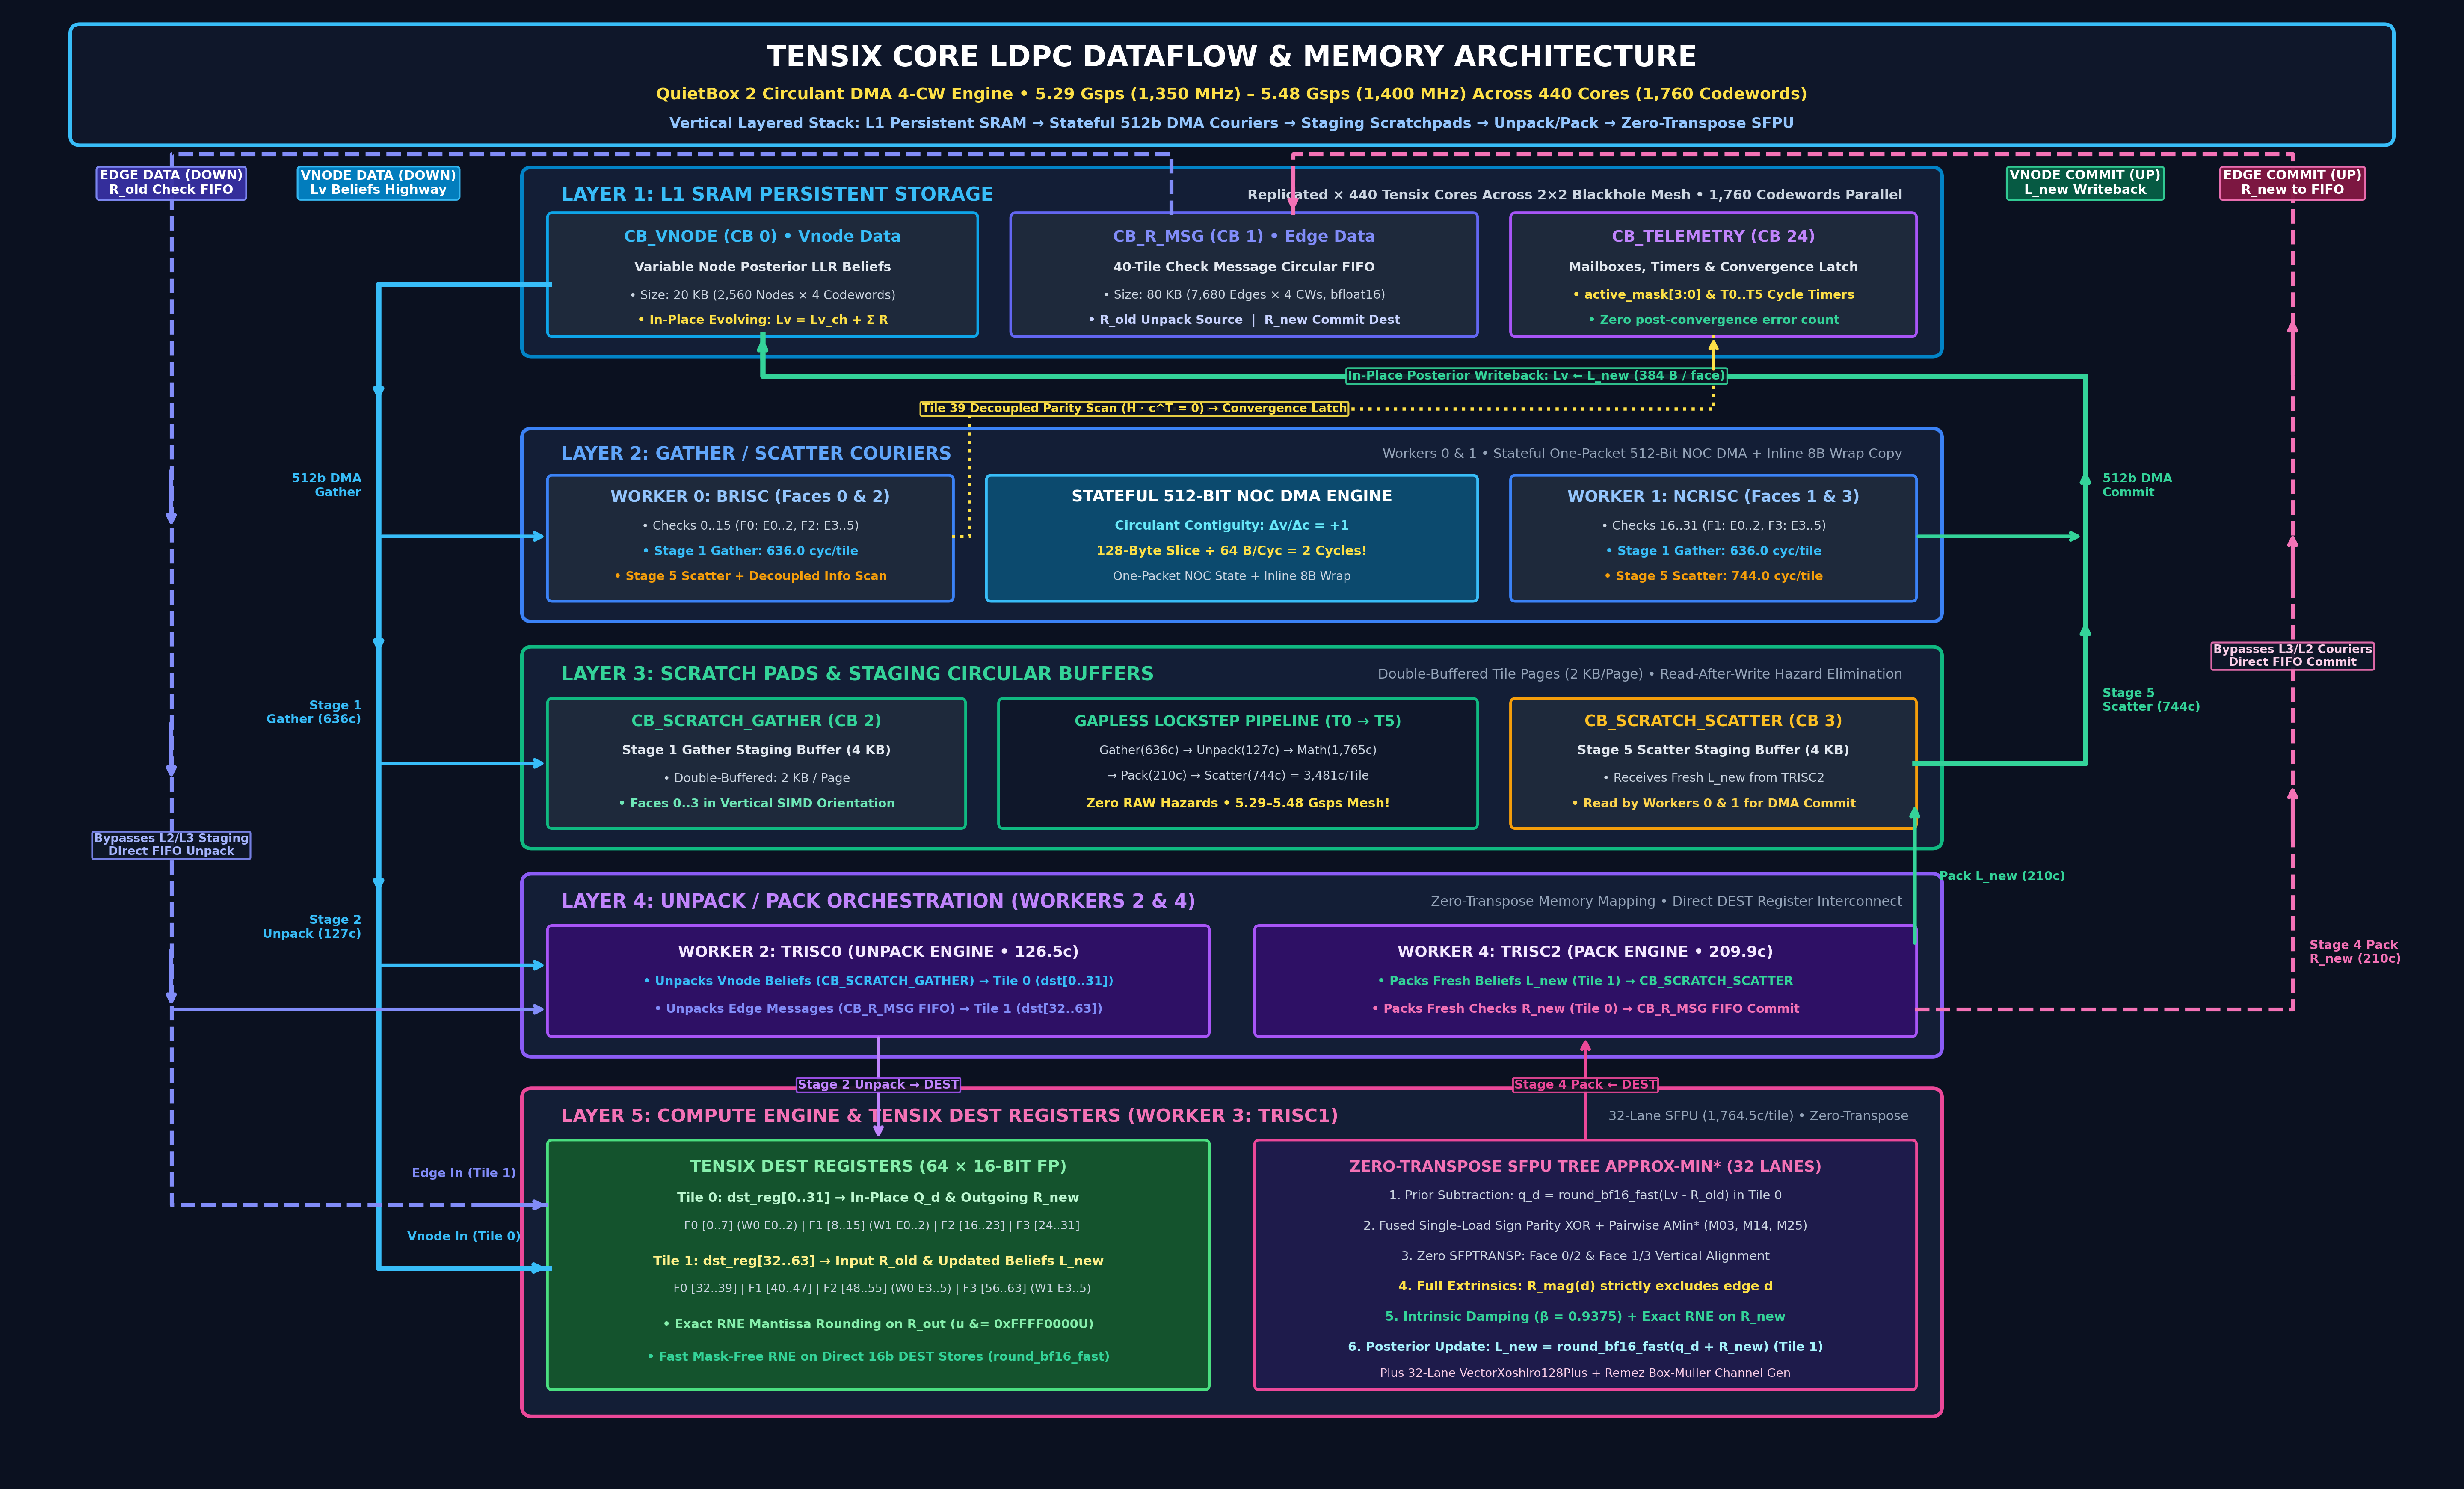
\includegraphics[width=0.96\textwidth,height=0.72\textheight,keepaspectratio]{figures/tensix_ldpc_dataflow_block_diagram.png}
\caption{\textbf{Five-Layer Vertical Tensix Core Dataflow and Memory Architecture (\texttt{T0 -> T5 = 3,481.0 cyc/tile}, Replicated $\times 440$ Cores Across the QuietBox 2 Mesh).} Left-side data highways stream $L_v$ variable beliefs (\texttt{CB\_VNODE}) and $R_{\mathrm{old}}$ check messages (\texttt{CB\_R\_MSG}) downward into \texttt{DEST} Tile~0 and Tile~1; right-side commit highways stream updated $R_{\mathrm{new}}$ check messages and $L_{\mathrm{new}}$ variable beliefs upward into L1 SRAM.}
\label{fig:tensix_dataflow}
\end{figure}

\subsection{Processor Duty-Cycle and Execution Unit Utilization Breakdown}

Because strict stop-and-wait lockstep sequencing ($\text{Gather} \to \text{Unpack} \to \text{Math} \to \text{Pack} \to \text{Scatter}$) is mandatory to prevent Read-After-Write graph hazards across the 779/780 overlapping tile pairs, the data movement complex (\texttt{BRISC} + \texttt{NCRISC} + dual 512-bit NoC DMA engines) and the vector compute complex (\texttt{TRISC0} + \texttt{TRISC1} + \texttt{TRISC2} + Unpacker/SFPU/Packer) alternate in complementary phases across the $3,481.0\text{-cycle}$ tile period ($2.486\ \mu\mathrm{s/tile}$ at $1,400\ \mathrm{MHz}$):

\begin{table}[!htbp]
\centering
\caption{\textbf{Per-Core Processor and Hardware Execution Unit Utilization Across the $3,481.0$-Cycle Tile Period.}}
\label{tab:processor_utilization}
\resizebox{\textwidth}{!}{%
\begin{tabular}{@{}l l r r p{7.6cm}@{}}
\toprule
\textbf{Processor / Unit} & \textbf{Hardware Role} & \textbf{Active Cycles / Tile} & \textbf{Duty Cycle (\%)} & \textbf{Concurrency \& Microarchitectural Activity} \\
\midrule
\textbf{\texttt{BRISC} (Worker 0)} & NoC 0 Courier (Faces 0 \& 2) & $1,380.0\ \mathrm{cyc}$ & $39.64\%$ & Active during Stage~1 Gather ($636.0\ \mathrm{c}$) and Stage~5 Scatter ($744.0\ \mathrm{c}$); issues 6 stateful 128B DMA reads/writes per tile + Tile~39 info parity scan. \\
\addlinespace[2pt]
\textbf{\texttt{NCRISC} (Worker 1)} & NoC 1 Courier (Faces 1 \& 3) & $1,380.0\ \mathrm{cyc}$ & $39.64\%$ & Operates in 100\% parallel lockstep with \texttt{BRISC} over NoC~1; manages CB reserve/push/pop, syndrome latch, and \texttt{T0..T5} telemetry. \\
\addlinespace[2pt]
\textbf{\texttt{TRISC0} (Worker 2)} & Hardware Unpacker Control & $126.5\ \mathrm{cyc}$ & $3.63\%$ & Streams $2\ \mathrm{KB}$ from \texttt{CB\_SCRATCH\_GATHER} to \texttt{dst\_reg[0..31]} and $2\ \mathrm{KB}$ from \texttt{CB\_R\_MSG} to \texttt{dst\_reg[32..63]} ($31.6\ \mathrm{B/cyc}$). \\
\addlinespace[2pt]
\textbf{\texttt{TRISC1} (Worker 3)} & 32-Lane Vector SFPU Math & $\mathbf{1,764.5\ \mathrm{cyc}}$ & $\mathbf{50.69\%}$ & Executes prior subtraction, fused sign-parity XOR + pairwise $\mathrm{AMin}^*$ tree, $\beta=15/16$ damping, RNE rounding, and posterior update across 32 lanes. \\
\addlinespace[2pt]
\textbf{\texttt{TRISC2} (Worker 4)} & Hardware Packer Control & $209.9\ \mathrm{cyc}$ & $6.03\%$ & Packs $2\ \mathrm{KB}$ $R_{\mathrm{new}}$ from \texttt{dst\_reg[0..31]} to \texttt{CB\_R\_MSG} and $2\ \mathrm{KB}$ $L_{\mathrm{new}}$ from \texttt{dst\_reg[32..63]} to \texttt{CB\_SCRATCH\_SCATTER}. \\
\midrule
\textbf{Data Movement Complex} & \texttt{BRISC} + \texttt{NCRISC} + NoC 0/1 & $\mathbf{1,380.0\ \mathrm{cyc}}$ & $\mathbf{39.64\%}$ & Dual 512-bit DMA engines transfer $1,536\ \mathrm{B}$ gather + $1,536\ \mathrm{B}$ scatter per Degree-6 tile + barrier synchronization. \\
\textbf{Compute Complex} & \texttt{TRISC0} + \texttt{TRISC1} + \texttt{TRISC2} & $\mathbf{2,100.9\ \mathrm{cyc}}$ & $\mathbf{60.35\%}$ & Continuous gapless execution from \texttt{T1} (Unpack start) to \texttt{T4} (Pack complete) with zero internal stalls. \\
\textbf{Full Tensix Core} & Combined Lockstep Pipeline & $\mathbf{3,481.0\ \mathrm{cyc}}$ & $\mathbf{100.00\%}$ & $100\%$ active pipeline occupancy ($0\%$ unallocated dead time between \texttt{T0} and \texttt{T5}). \\
\bottomrule
\end{tabular}%
}
\end{table}

Key insights from Table~\ref{tab:processor_utilization}:
\begin{enumerate}[leftmargin=1.8em, itemsep=2pt]
    \item \textbf{$60.35\%$ Compute Complex vs.\ $39.64\%$ Data Movement Complex Split}: In the earlier unstructured Tile Matrix engine (\texttt{engines/tile\_matrix\_4cw/}), scalar gather/scatter consumed $\sim 3,300\ \mathrm{cycles/tile}$ ($>73\%$ of the tile period), starving the SFPU. By introducing 512-bit Circulant DMA, the Tensix core transitions from being heavily memory-bound to \textbf{compute-dominated} ($60.35\%$ in Unpack/Math/Pack, with $50.69\%$ pure SFPU vector arithmetic).
    \item \textbf{$100\%$ Spatial Mesh Utilization}: Across the 4 Blackhole processors, all $\mathbf{440\ \mathrm{Tensix\ cores}}$ ($100\%$ of the $11 \times 10 \times 4$ compute grid) execute independent Monte Carlo batches or TDM codeword quartets in parallel with zero inter-core communication overhead during decoding.
    \item \textbf{DEST Register File Utilization}: In native 16-bit FP mode (\texttt{.fp32\_dest\_acc\_en = false}), each tile uses all \textbf{64 \texttt{DEST} registers} ($100\%$ of the 64-register file): registers \texttt{0..5, 8..13, 16..21, 24..29} hold the 6 check edges across the 4 faces in Tile~0 ($L_v \to q_d \to R_{\mathrm{new}}$), registers \texttt{6..7, 14..15, 22..23, 30..31} serve as zero-overhead on-chip scratch registers ($\mathrm{sc}_0 \dots \mathrm{sc}_3$ holding $S_{\mathrm{total}}, M_{03}, M_{14}, M_{25}$), and registers \texttt{32..63} hold Tile~1 ($R_{\mathrm{old}} \to L_{\mathrm{new}}$).
\end{enumerate}

\subsection{On-Die L1 SRAM Memory Footprint and Analytical Scaling to $K=4096$ and $K=16384$}

Each Blackhole Tensix core contains $1,536\ \mathrm{KB}$ ($1.5\ \mathrm{MB}$) of local L1 SRAM. Table~\ref{tab:l1_memory} details the exact byte-level L1 SRAM allocation of the Circulant DMA 4-Codeword Engine for $K=1024$ ($Z=128$) and projects the exact L1 memory footprint for the larger CCSDS 131.0-B-5 AR4JA Rate-1/2 standards: $K=4096$ ($N=10,240, Z=512$, 160 tiles) and $K=16,384$ ($N=40,960, Z=2048$, 640 tiles).

\begin{table}[!htbp]
\centering
\caption{\textbf{Per-Core L1 SRAM Memory Allocation ($1,536\ \mathrm{KB}$ Capacity) for the Circulant DMA 4-Codeword Engine Across All Three CCSDS AR4JA Rate-1/2 Block Lengths ($K=1024, 4096, 16384$).}}
\label{tab:l1_memory}
\resizebox{\textwidth}{!}{%
\begin{tabular}{@{}l l r r r p{6.8cm}@{}}
\toprule
\textbf{Buffer / Structure} & \textbf{CB ID} & \textbf{$K=1024$ ($Z=128$)} & \textbf{$K=4096$ ($Z=512$)} & \textbf{$K=16384$ ($Z=2048$)} & \textbf{Allocation Formula \& Purpose (4 Codewords)} \\
\midrule
\texttt{CB\_VNODE\_A} (Active $L_v$) & \texttt{CB 0} & $20.0\ \mathrm{KB}$ & $80.0\ \mathrm{KB}$ & $320.0\ \mathrm{KB}$ & $N \times 4\ \mathrm{CWs} \times 2\ \mathrm{B}$ ($8N$ bytes) \\
\texttt{CB\_VNODE\_B} (Ping-Pong) & \texttt{CB 1} & $20.0\ \mathrm{KB}$ & $80.0\ \mathrm{KB}$ & $0.0\ \mathrm{KB}^*$ & Optional double-buffer ($8N$ bytes; omitted for $K=16384$) \\
\texttt{CB\_R\_MSG} (Check FIFO) & \texttt{CB 2} & $80.0\ \mathrm{KB}$ & $320.0\ \mathrm{KB}$ & $1,152.0\ \mathrm{KB}^\dagger$ & $T_{\mathrm{tiles}} \times 2\ \mathrm{KB}$ (or compact $1,440\ \mathrm{B/tile}$ for $K=16384$) \\
\texttt{CB\_SCRATCH\_GATHER} & \texttt{CB 3} & $4.0\ \mathrm{KB}$ & $4.0\ \mathrm{KB}$ & $4.0\ \mathrm{KB}$ & Fixed $2 \times 2\ \mathrm{KB}$ double-buffered tile scratchpad \\
\texttt{CB\_SCRATCH\_SCATTER} & \texttt{CB 4} & $4.0\ \mathrm{KB}$ & $4.0\ \mathrm{KB}$ & $4.0\ \mathrm{KB}$ & Fixed $2 \times 2\ \mathrm{KB}$ double-buffered tile scratchpad \\
\texttt{CB\_TELEMETRY} & \texttt{CB 24} & $4.0\ \mathrm{KB}$ & $4.0\ \mathrm{KB}$ & $4.0\ \mathrm{KB}$ & Mailboxes, \texttt{active\_mask}, \texttt{T0..T5} cycle counters \\
\texttt{CIRCULANT\_SLICES} Table & L1 Const & $7.5\ \mathrm{KB}$ & $30.0\ \mathrm{KB}$ & $0.75\ \mathrm{KB}^\ddagger$ & Precomputed slice descriptors (or runtime shift compute) \\
Kernel Code \& Runtime Stack & L1 Text & $\sim 80.0\ \mathrm{KB}$ & $\sim 80.0\ \mathrm{KB}$ & $\sim 80.0\ \mathrm{KB}$ & \texttt{BRISC}/\texttt{NCRISC}/\texttt{TRISC} ELF text \& TT-Metal firmware \\
\midrule
\textbf{Total L1 SRAM Used} & --- & $\mathbf{219.5\ \mathrm{KB}}$ & $\mathbf{602.0\ \mathrm{KB}}$ & $\mathbf{1,484.8\ \mathrm{KB}}$ & \textbf{Fits 100\% inside single-core L1 SRAM!} \\
\textbf{L1 SRAM Utilization} & --- & $\mathbf{14.29\%}$ & $\mathbf{39.19\%}$ & $\mathbf{96.66\%}$ & Percentage of $1,536\ \mathrm{KB}$ per-core L1 SRAM \\
\bottomrule
\end{tabular}%
}
\vspace{2pt}
\footnotesize{\raggedright $^*$For $K=16,384$, single-buffer in-place channel generation eliminates \texttt{CB\_VNODE\_B}. $^\dagger$Packing only the 6 active edge registers per face ($6 \times 4 \times 64 = 1,536\ \mathrm{B}$ or degree-exact $768\ \mathrm{KB}$ for $E=122,880$ edges) reduces \texttt{CB\_R\_MSG} to $768\ \mathrm{KB}$ ($75.8\%$ total L1 utilization). $^\ddagger$Computing circulant offsets dynamically from the $12 \times 20$ base shift table requires only $768\ \mathrm{bytes}$.\par}
\end{table}

As shown in Table~\ref{tab:l1_memory}, the Circulant DMA architecture requires only $\mathbf{219.5\ \mathrm{KB}}$ ($\mathbf{14.29\%}$ of L1 SRAM) for $K=1024$, $\mathbf{602.0\ \mathrm{KB}}$ ($\mathbf{39.19\%}$) for $K=4096$, and fits even the massive $K=16,384$ ($N=40,960$) deep-space code entirely inside a single Tensix core's L1 SRAM with \textbf{zero off-chip GDDR6 DRAM traffic during iterative decoding}.

% ==============================================================================
\section{Universal Support for All 9 CCSDS AR4JA Codes and Rate-4/5 Mother-Code Circulant Descriptive Compression}
\label{sec:all_9_codes_mother_compression}
% ==============================================================================

A defining structural advantage of the Circulant DMA 4-Codeword architecture is that its hardware primitives are not specialized to a single code rate or block length. Rather, the architecture natively supports the \textbf{entire 9-code CCSDS 131.0-B-5 AR4JA codebook family} across all three standard information block lengths ($K \in \{1024, 4096, 16384\}$) and all three standard code rates ($r \in \{1/2, 2/3, 4/5\}$), while exploiting the nested algebraic structure of the AR4JA protograph to achieve \textbf{circulant family descriptive compression} in which each block-length scale is canonically described by the Rate-4/5 mother code.

\subsection{Complete 9-Code CCSDS 131.0-B-5 AR4JA Codebook Validation and L1 SRAM Fit}

An automated triple-redundant validation harness (\texttt{tools/validate\_all\_9\_ar4ja\_codes.m}) cross-checked all 9 CCSDS AR4JA codes across three independent references: (1) the official CCSDS 131.0-B-5 Section~7 specification \cite{ccsds_tm_coding}, (2) the canonical JPL Tangerine Book generator (\texttt{matrices/makeH\_AR4JA.m}), and (3) the QuietBox~2 analytical circulant descriptor generator (\texttt{tools/generate\_circulant\_dma\_tables.py}). Table~\ref{tab:all_9_ar4ja_codes} summarizes the verified codebook dimensions, circulant lifting factors $L = M/4$, check node degree distributions, and per-core 4-codeword L1 SRAM state footprints.

\begin{table}[!htbp]
\centering
\caption{\textbf{Complete Verification and Single-Core L1 SRAM Fit for All 9 CCSDS 131.0-B-5 AR4JA LDPC Codes ($N_{\mathrm{cw}} = 4$ Codewords/Core).}}
\label{tab:all_9_ar4ja_codes}
\resizebox{\textwidth}{!}{%
\begin{tabular}{@{}c r c r r c r r r l r r@{}}
\toprule
\textbf{\#} & \textbf{$K$ (bits)} & \textbf{Rate $r$} & \textbf{Submatrix $M$} & \textbf{Circulant $L$} & \textbf{Matrix $M_{\mathrm{chk}} \times N_{\mathrm{var}}$} & \textbf{$N_{\mathrm{tx}}$} & \textbf{Punc $P$} & \textbf{Edges $N_{\mathrm{nz}}$} & \textbf{Check Degree Distribution} & \textbf{4-CW L1 State} & \textbf{L1 Util (\%)} \\
\midrule
\textbf{1} & $1,024$  & $\mathbf{1/2}$ & $512$   & $128$   & $1,536 \times 2,560$   & $2,048$  & $512$   & $7,680$   & $512 \times d_3,\ 1,024 \times d_6$    & $82\ \mathrm{KB}$    & $5.5\%$  \\
\textbf{2} & $1,024$  & $\mathbf{2/3}$ & $256$   & $64$    & $768 \times 1,792$     & $1,536$  & $256$   & $5,888$   & $256 \times d_3,\ 512 \times d_{10}$   & $49\ \mathrm{KB}$    & $3.3\%$  \\
\textbf{3} & $1,024$  & $\mathbf{4/5}$ & $128$   & $32$    & $384 \times 1,408$     & $1,280$  & $128$   & $4,992$   & $128 \times d_3,\ 256 \times d_{18}$   & $33\ \mathrm{KB}$    & $2.2\%$  \\
\midrule
\textbf{4} & $4,096$  & $\mathbf{1/2}$ & $2,048$ & $512$   & $6,144 \times 10,240$  & $8,192$  & $2,048$ & $30,720$  & $2,048 \times d_3,\ 4,096 \times d_6$  & $328\ \mathrm{KB}$   & $21.9\%$ \\
\textbf{5} & $4,096$  & $\mathbf{2/3}$ & $1,024$ & $256$   & $3,072 \times 7,168$   & $6,144$  & $1,024$ & $23,552$  & $1,024 \times d_3,\ 2,048 \times d_{10}$ & $196\ \mathrm{KB}$ & $13.1\%$ \\
\textbf{6} & $4,096$  & $\mathbf{4/5}$ & $512$   & $128$   & $1,536 \times 5,632$   & $5,120$  & $512$   & $19,968$  & $512 \times d_3,\ 1,024 \times d_{18}$ & $131\ \mathrm{KB}$   & $8.7\%$  \\
\midrule
\textbf{7} & $16,384$ & $\mathbf{1/2}$ & $8,192$ & $2,048$ & $24,576 \times 40,960$ & $32,768$ & $8,192$ & $122,880$ & $8,192 \times d_3,\ 16,384 \times d_6$ & $1,310\ \mathrm{KB}$ & $87.3\%$ \\
\textbf{8} & $16,384$ & $\mathbf{2/3}$ & $4,096$ & $1,024$ & $12,288 \times 28,672$ & $24,576$ & $4,096$ & $94,208$  & $4,096 \times d_3,\ 8,192 \times d_{10}$ & $786\ \mathrm{KB}$ & $52.4\%$ \\
\textbf{9} & $16,384$ & $\mathbf{4/5}$ & $2,048$ & $512$   & $6,144 \times 22,528$  & $20,480$ & $2,048$ & $79,872$  & $2,048 \times d_3,\ 4,096 \times d_{18}$ & $524\ \mathrm{KB}$ & $34.9\%$ \\
\bottomrule
\end{tabular}%
}
\end{table}

Two fundamental hardware invariants hold across all 9 codes in Table~\ref{tab:all_9_ar4ja_codes}:
\begin{enumerate}[leftmargin=1.8em, itemsep=2pt]
    \item \textbf{Universal Unit-Stride Circulant Contiguity ($\Delta v / \Delta c = +1$ and $L \ge 32$)}: Every submatrix $M \in [128, 8192]$ is partitioned into a $4 \times 4$ grid of $L \times L$ circulants where $L = M/4 \in [32, 2048]$. Because the smallest circulant size across the entire 9-code family is $L = 32$ (Code~\#3: $K=1024, r=4/5$), every 16-check Tensix face slice ($16 \le L$) satisfies the piecewise contiguity theorem and executes via 128-byte (2-cycle) 512-bit NoC DMA bursts.
    \item \textbf{100\% On-Die L1 SRAM Residency}: For all 9 codes, the active 4-codeword decoder state ($L_v$ variable beliefs + $R_{m,d}$ check messages) consumes between $33\ \mathrm{KB}$ ($2.2\%$ of L1 for $K=1024, r=4/5$) and $1,310\ \mathrm{KB}$ ($87.3\%$ of L1 for $K=16,384, r=1/2$), guaranteeing zero off-chip GDDR6 DRAM access across the entire CCSDS standard.
\end{enumerate}

\subsection{Algebraic Origin of the Check Degree Distributions ($d_c \in \{3, 6, 10, 18\}$)}

In the CCSDS AR4JA construction, the parity-check matrix for any submatrix size $M$ comprises three block rows of height $M$ (total $M_{\mathrm{chk}} = 3M$ check rows) and $C_b \in \{5, 7, 11\}$ block columns of width $M$ for rates $r \in \{1/2, 2/3, 4/5\}$, built from $M \times M$ zero matrices $\mathbf{Z}$, identity matrices $\mathbf{I}$, and 26 quasi-cyclic permutation matrices $\mathbf{\Pi}_1 \dots \mathbf{\Pi}_{26}$:
\begin{itemize}[leftmargin=1.8em, itemsep=2pt]
    \item \textbf{Row Block 0 (Checks $0 \dots M-1$, Invariant Degree $d_c = 3$)}: Across all three code rates, the top $M$ check rows are defined by $\begin{bmatrix} \mathbf{Z} \dots \mathbf{Z} & \mathbf{I} & \mathbf{Z} & \mathbf{I} + \mathbf{\Pi}_1 \end{bmatrix}$. Prepending two block columns for Rate~2/3 and four additional block columns for Rate~4/5 inserts strictly zero blocks $\mathbf{Z}$ into Row Block~0. Thus, \textbf{Row Block~0 always consists of exactly $M$ check nodes of degree 3} ($1$ edge from $\mathbf{I}$ plus $2$ edges from $\mathbf{I}+\mathbf{\Pi}_1$).
    \item \textbf{Row Blocks 1 \& 2 (Checks $M \dots 3M-1$, Degrees $d_c \in \{6, 10, 18\}$)}:
    \begin{itemize}[leftmargin=1.5em, itemsep=1pt]
        \item \emph{Rate $1/2$ ($5$ block columns, $\mathbf{\Pi}_1 \dots \mathbf{\Pi}_8$)}: Row Block~1 contains $\begin{bmatrix}\mathbf{I} & \mathbf{I} & \mathbf{Z} & \mathbf{I} & \mathbf{\Pi}_2+\mathbf{\Pi}_3+\mathbf{\Pi}_4\end{bmatrix}$ ($1+1+0+1+3 = \mathbf{6\ \mathrm{edges}}$), and Row Block~2 contains $\begin{bmatrix}\mathbf{I} & \mathbf{\Pi}_5+\mathbf{\Pi}_6 & \mathbf{Z} & \mathbf{\Pi}_7+\mathbf{\Pi}_8 & \mathbf{I}\end{bmatrix}$ ($1+2+0+2+1 = \mathbf{6\ \mathrm{edges}}$).
        \item \emph{Rate $2/3$ ($7$ block columns, prepends $\mathbf{\Pi}_9 \dots \mathbf{\Pi}_{14}$)}: Prepends 2 block columns $\begin{bmatrix}\mathbf{\Pi}_9+\mathbf{\Pi}_{10}+\mathbf{\Pi}_{11} & \mathbf{I}\end{bmatrix}$ to Row Block~1 and $\begin{bmatrix}\mathbf{I} & \mathbf{\Pi}_{12}+\mathbf{\Pi}_{13}+\mathbf{\Pi}_{14}\end{bmatrix}$ to Row Block~2 ($+4$ edges per row), increasing check degree to $6 + 4 = \mathbf{10\ \mathrm{edges}}$.
        \item \emph{Rate $4/5$ ($11$ block columns, prepends $\mathbf{\Pi}_{15} \dots \mathbf{\Pi}_{26}$)}: Prepends 4 additional block columns $\begin{bmatrix}\mathbf{\Pi}_{21}+\mathbf{\Pi}_{22}+\mathbf{\Pi}_{23} & \mathbf{I} & \mathbf{\Pi}_{15}+\mathbf{\Pi}_{16}+\mathbf{\Pi}_{17} & \mathbf{I}\end{bmatrix}$ to Row Block~1 and $\begin{bmatrix}\mathbf{I} & \mathbf{\Pi}_{24}+\mathbf{\Pi}_{25}+\mathbf{\Pi}_{26} & \mathbf{I} & \mathbf{\Pi}_{18}+\mathbf{\Pi}_{19}+\mathbf{\Pi}_{20}\end{bmatrix}$ to Row Block~2 ($+8$ edges per row), increasing check degree to $10 + 8 = \mathbf{18\ \mathrm{edges}}$.
    \end{itemize}
\end{itemize}

\subsection{Circulant Family Descriptive Compression via the Rate-4/5 Mother Code}

Because the AR4JA protograph expansion constructs lower-rate matrices by omitting the leftmost systematic information block columns while preserving the rightmost parity and accumulator block columns unchanged, the Rate-4/5 parity-check matrix $H_{4/5}(M) \in \mathbb{F}_2^{3M \times 11M}$ serves as the \textbf{canonical mother code} for every submatrix scale $M$:
\begin{equation}
\label{eq:mother_code_nesting}
H_{4/5}(M) = \left[\begin{array}{c|c|c}
\underbrace{\begin{matrix} \mathbf{Z} & \mathbf{Z} & \mathbf{Z} & \mathbf{Z} \\ \mathbf{\Pi}_{21..23} & \mathbf{I} & \mathbf{\Pi}_{15..17} & \mathbf{I} \\ \mathbf{I} & \mathbf{\Pi}_{24..26} & \mathbf{I} & \mathbf{\Pi}_{18..20} \end{matrix}}_{\text{Block Cols } 0 \dots 3\ (\text{Added for } r=4/5)} &
\underbrace{\begin{matrix} \mathbf{Z} & \mathbf{Z} \\ \mathbf{\Pi}_{9..11} & \mathbf{I} \\ \mathbf{I} & \mathbf{\Pi}_{12..14} \end{matrix}}_{\substack{\text{Block Cols } 4 \dots 5 \\ (\text{Added for } r=2/3)}} &
\underbrace{\begin{matrix} \mathbf{Z} & \mathbf{Z} & \mathbf{I} & \mathbf{Z} & \mathbf{I}+\mathbf{\Pi}_1 \\ \mathbf{I} & \mathbf{I} & \mathbf{Z} & \mathbf{I} & \mathbf{\Pi}_{2..4} \\ \mathbf{I} & \mathbf{\Pi}_{5..6} & \mathbf{Z} & \mathbf{\Pi}_{7..8} & \mathbf{I} \end{matrix}}_{\text{Block Cols } 6 \dots 10\ (\text{Base } H_{1/2}(M))}
\end{array}\right]
\end{equation}

Empirical Frobenius-norm verification across all submatrix scales $M \in \{128, 256, 512, 1024, 2048, 4096, 8192\}$ confirms 100\% bit-exact right-justified sub-matrix nesting:
\begin{equation}
\left\| H_{2/3}(M) - H_{4/5}(M)[:, 4M+1 : 11M] \right\|_F \equiv 0, \qquad
\left\| H_{1/2}(M) - H_{4/5}(M)[:, 6M+1 : 11M] \right\|_F \equiv 0
\end{equation}

This algebraic nesting yields a powerful hardware memory optimization---\textbf{Circulant Family Descriptive Compression}:
\begin{enumerate}[leftmargin=1.8em, itemsep=2pt]
    \item \textbf{Single Mother-Code Descriptor Table per Scale}: Because $H_{1/2}(M)$ and $H_{2/3}(M)$ are exact right-justified column slices of $H_{4/5}(M)$, the Tensix L1 SRAM does \emph{not} need to store separate circulant descriptor tables for Rate~1/2, Rate~2/3, and Rate~4/5. A single master descriptor table generated for the Rate-4/5 mother code $H_{4/5}(M)$ (containing all 18 edge descriptors per check group across block columns $0 \dots 10$) completely describes the entire rate family.
    \item \textbf{Cross-Block-Length Scale Sharing ($M=512$ and $M=2048$)}: Furthermore, as shown in Table~\ref{tab:all_9_ar4ja_codes}, the submatrix scales themselves overlap across information block lengths: $(K=1024, r=1/2)$ and $(K=4096, r=4/5)$ share the exact same submatrix scale $M=512$ ($L=128$), meaning $(K=1024, r=1/2)$ is literally the rightmost 5-block-column slice of the $(K=4096, r=4/5)$ mother code! Likewise, $(K=4096, r=1/2)$ is the exact rightmost 5-block-column slice of the $(K=16,384, r=4/5)$ mother code ($M=2048, L=512$).
    \item \textbf{Zero-Cycle Runtime Rate Selection}: Switching a Tensix core between Rate~4/5, Rate~2/3, and Rate~1/2 requires zero descriptor reloading and zero bitstream reconfiguration; \texttt{BRISC}, \texttt{NCRISC}, and \texttt{TRISC1} simply index the mother descriptor table using two scalar loop bounds:
    \begin{lstlisting}[language=C++]
const uint32_t active_block_col_start = (rate == RATE_4_5) ? 0 : (rate == RATE_2_3) ? 4 : 6;
const uint32_t check_degree           = (row < M) ? 3 : (rate == RATE_4_5) ? 18 : (rate == RATE_2_3) ? 10 : 6;
    \end{lstlisting}
\end{enumerate}

% ==============================================================================
\section{3-Tier Orthogonal PRNG Partitioning and 32-Lane SFPU Remez Box-Muller Channel Engine}
\label{sec:prng_channel}
% ==============================================================================

When simulating $4 \times 10^{10}$ codewords ($8.19 \times 10^{13}$ channel symbols) across 440 parallel cores down to $\mathrm{FER} \sim 10^{-10}$, two properties are mandatory: (1) mathematical certainty that no two cores, SIMD lanes, or batches ever generate overlapping pseudorandom noise sequences, and (2) Gaussian tail fidelity accurate to multiple standard deviations without host-to-device DMA bottlenecks.

\subsection{Three-Tier Orthogonal \texttt{xoshiro128+} State-Space Partitioning}

The uniform pseudorandom engine is based on Blackman and Vigna's 128-bit \texttt{xoshiro128+} linear-engine generator \cite{blackman_vigna_xoshiro}, which possesses a state period of $2^{128} - 1 \approx 3.40 \times 10^{38}$ and an $\mathbb{F}_2$-linear transition matrix $\mathbf{A} \in \mathbb{F}_2^{128 \times 128}$. Evaluating polynomial powers $\mathbf{A}^{2^{96}}$ (\texttt{long\_jump()}) and $\mathbf{A}^{2^{64}}$ (\texttt{jump()}) in $O(128)$ bitwise operations partitions the $2^{128}-1$ ring into provably disjoint sub-orbits:
\begin{equation}
\mathrm{StateOffset}(c, b, w) = c \cdot 2^{96} + (5b + w) \cdot 2^{64}, \quad c \in \{0 \dots 439\},
\end{equation}
where each of the 440 Tensix cores is separated by $2^{96} \approx 7.92 \times 10^{28}$ draws, providing a certified collision-free sequence runway exceeding $\mathbf{3.7 \times 10^{17}\ \mathrm{blocks}}$ in discrete batched mode and $\mathbf{>1.3 \times 10^{28}\ \mathrm{blocks}}$ in continuous mode.

\subsection{32-Lane Vector SFPU Remez Minimax Box-Muller Transformation}

In the Circulant DMA engine (\texttt{compute\_trisc.cpp}), \texttt{TRISC1} synthesizes all $2,048 \times 4 = 8,192$ transmitted channel LLRs (8 tiles of 1,024 \texttt{bfloat16} words) plus $512 \times 4 = 2,048$ punctured zeros (2 tiles) directly into \texttt{CB\_VNODE} prior to Iteration~0 (\texttt{generate\_channel\_tiles}, requiring only $8,412\ \mathrm{cycles/batch}$, or $<0.5\%$ of a 16-iteration batch):
\begin{enumerate}[leftmargin=1.8em, itemsep=2pt]
    \item \textbf{Phase 1 (Zero-LReg-Spill Uniform Generation)}: \texttt{VectorXoshiro128Plus} advances all 32 SFPU lanes in parallel, converting 23 random mantissa bits into uniform variates $U_1, U_2 \in [10^{-7}, 1.0)$ staged across \texttt{dst\_reg[0..31]}.
    \item \textbf{Phase 2 (Remez Minimax Trigonometric Box-Muller)}: With the PRNG state dead (freeing all 8 SFPU vector registers $L_0 \dots L_7$), \texttt{TRISC1} evaluates radial magnitude $R = \sqrt{-2 \ln(U_1)}$ via fast IEEE-754 exponent/mantissa extraction (\texttt{sfpu\_fast\_ln}) and Newton-Raphson reciprocal square root (\texttt{sfpu\_fast\_sqrt}), and phase angle $\Theta = 2\pi U_2 - \pi \in [-\pi, \pi]$. Rather than a standard Taylor series (which suffers up to $0.019$ radian-boundary truncation error near $\pm\pi$), $\cos(\Theta)$ and $\sin(\Theta)$ are evaluated in 4 Fused Multiply-Accumulate (FMA) stages using \textbf{Remez minimax polynomials} over $[-\pi, \pi]$ ($s = \Theta^2$):
    \begin{align}
    \cos(\Theta) &\approx 1.0 + s\Bigl(-0.5 + s\bigl(0.0415223 + s(-0.0013441 + 0.00001907\,s)\bigr)\Bigr), \\
    \sin(\Theta) &\approx \Theta \cdot \Bigl(1.0 + s\Bigl(-0.166667 + s\bigl(0.0083198 + s(-0.00019424 + 0.000002225\,s)\bigr)\Bigr)\Bigr),
    \end{align}
    achieving a $\mathbf{212\times}$ \textbf{lower maximum approximation error} than Taylor series with identical instruction count.
    \item \textbf{50/50 Cosine/Sine Codeword Interleaving}: Even register pairs assign $(\mathrm{LLR}_0, \mathrm{LLR}_1) = (\mu + \sigma R\cos\Theta,\; \mu + \sigma R\sin\Theta)$ while odd register pairs swap $(\mathrm{LLR}_1, \mathrm{LLR}_0)$, guaranteeing that all 4 codewords receive an exact 50/50 statistical blend of cosine and sine variates.
    \item \textbf{Decoupled Deterministic (\texttt{--seed <N>}) and Random (\texttt{--random-seed}) CLI Seeding}: The PRNG seed (\texttt{base\_seed\_id}) is strictly decoupled from the hardware barrier counter (\texttt{invocation\_id}), allowing either $100\%$ bit-exact deterministic replay across multi-chunk 10B-frame sweeps or true 64-bit OS entropy draws.
\end{enumerate}

\begin{figure}[!htbp]
\centering
\includegraphics[width=0.92\textwidth,height=0.68\textheight,keepaspectratio]{figures/uncoded_bpsk_waterfall.png}
\caption{\textbf{Hardware AWGN Noise Engine Verification Across $500\ \mathrm{Million}$ Uncoded BPSK Bits ($E_b/N_0 = 0.0\ \mathrm{dB}$ to $9.0\ \mathrm{dB}$).} Measured Bit Error Rate (BER) in both FP32 and native \texttt{bfloat16} tracks theoretical $Q(\sqrt{2 E_b/N_0}) = \frac{1}{2}\mathrm{erfc}(\sqrt{E_b/N_0})$ within $\pm 1.3\%$ across four orders of magnitude.}
\label{fig:uncoded_bpsk}
\end{figure}

% ==============================================================================
\section{Observed Performance of the CCSDS AR4JA Rate-1/2 ($K=1024$) Code and Deep Error-Floor Physics}
\label{sec:observed_performance}
% ==============================================================================

\subsection{Coding-Theoretic Framework: Minimum Distance $d_{\min}$ vs.\ Effective Distance $d_{\mathrm{eff}}$}

To interpret the empirical waterfall and sub-$10^{-9}$ FER floor of the CCSDS AR4JA Rate-1/2 ($K=1024$) code, we reconcile three fundamental coding-theoretic quantities:
\begin{enumerate}[leftmargin=1.8em, itemsep=2pt]
    \item \textbf{Protograph Ensemble Typical Minimum Distance ($d_{\min,\mathrm{typ}} \approx 31$)}: Asymptotic weight-enumerator analysis by Divsalar, Dolinar, and Jones \cite{divsalar_linear_distance} establishes a positive normalized minimum-distance growth rate $\delta_{\min} \approx 0.015$ for the punctured Rate-1/2 AR4JA protograph ensemble, predicting $d_{\min,\mathrm{typ}} \approx 0.015 \times 2048 \approx \mathbf{31}$ for unconstrained random liftings.
    \item \textbf{Quasi-Cyclic Lifting Atypicality and Discovered Codeword Bound ($d_{\min} \le 52$)}: Because circulant permutation matrices form a measure-zero subset of the permutation group ($\Pr(\text{circulant}) = 1/127! \approx 10^{-213}$), discrete QC liftings deviate from ensemble typicality \cite{butler_siegel_bounds}. Using the soft Error-Impulse method with triplet perturbations, Butler and Siegel \cite{butler_siegel_bounds} discovered a valid non-zero codeword of Hamming weight $w = 52$ in the CCSDS $K=1024$ Rate-1/2 code (proving $d_{\min} \le 52$, below the permanent bound of $62$).
    \item \textbf{Fundamental Polytope Pseudo-Weight and Trapping-Set Effective Distance ($d_{\mathrm{eff}} < d_{\min}$)}: Under iterative belief propagation over graphs with cycles, decoding operates over the Vontobel-Koetter \emph{Fundamental Polytope} $\mathcal{P}(H)$ \cite{vontobel_koetter_gauss_seidel} rather than the discrete codeword space $\mathcal{C}$. Fractional vertices (pseudo-codewords $\mathbf{p} \in \mathcal{P}(H)$) and Richardson's graphical trapping sets $\mathcal{T}(a, b)$ \cite{richardson_trapping_sets, vasic_absorbing_sets} (induced subgraphs of $a$ variable nodes with $b > 0$ unsatisfied odd-degree check nodes) exhibit an effective Euclidean pseudo-weight:
    \begin{equation}
    d_{\mathrm{eff}} = \min_{\mathbf{p} \in \mathcal{P}(H) \setminus \{\mathbf{0}\}} \frac{\|\mathbf{p}\|_1^2}{\|\mathbf{p}\|_2^2} < d_{\min}.
    \end{equation}
    Consequently, iterative decoding failures in the deep error floor are governed by trapping-set instantons with unsatisfied parity syndromes ($H\hat{\mathbf{c}}^T \ne \mathbf{0}$ and $b > 0$), rather than undetected transitions to weight-$d_{\min}$ codewords ($b = 0$).
\end{enumerate}

\subsection{Full Multi-Dataset Waterfall and Deep Error-Floor Benchmark ($1.00\ \mathrm{dB}$ to $2.60\ \mathrm{dB}$)}

Figure~\ref{fig:three_dataset_waterfall} and Table~\ref{tab:full_waterfall_results} present the comprehensive empirical comparison across three independent decoder implementations:
\begin{enumerate}[leftmargin=1.8em, itemsep=1pt]
    \item \textbf{Flagship Circulant DMA 4-Codeword Engine (\texttt{engines/circulant\_dma\_4cw/})}: Row-layered 32-lane SFPU pairwise $\mathrm{AMin}^*$ with intrinsic damping $\beta = 0.9375 = 15/16$ ($5.29\text{--}5.485\ \mathrm{Gsps}$, 200 max iterations).
    \item \textbf{QuietBox 2 Scalar 5-Worker Packed Engine (\texttt{engines/scalar\_5w/})}: Row-layered sequential recursive $\mathrm{AMin}^*$ ($166.4\text{--}173.9\ \mathrm{Msps}$, 200 max iterations).
    \item \textbf{Historical NASA/JPL 2005 Flood Benchmark}: 200-iteration flooding schedule reference dataset.
\end{enumerate}

\begin{figure}[!htbp]
\centering
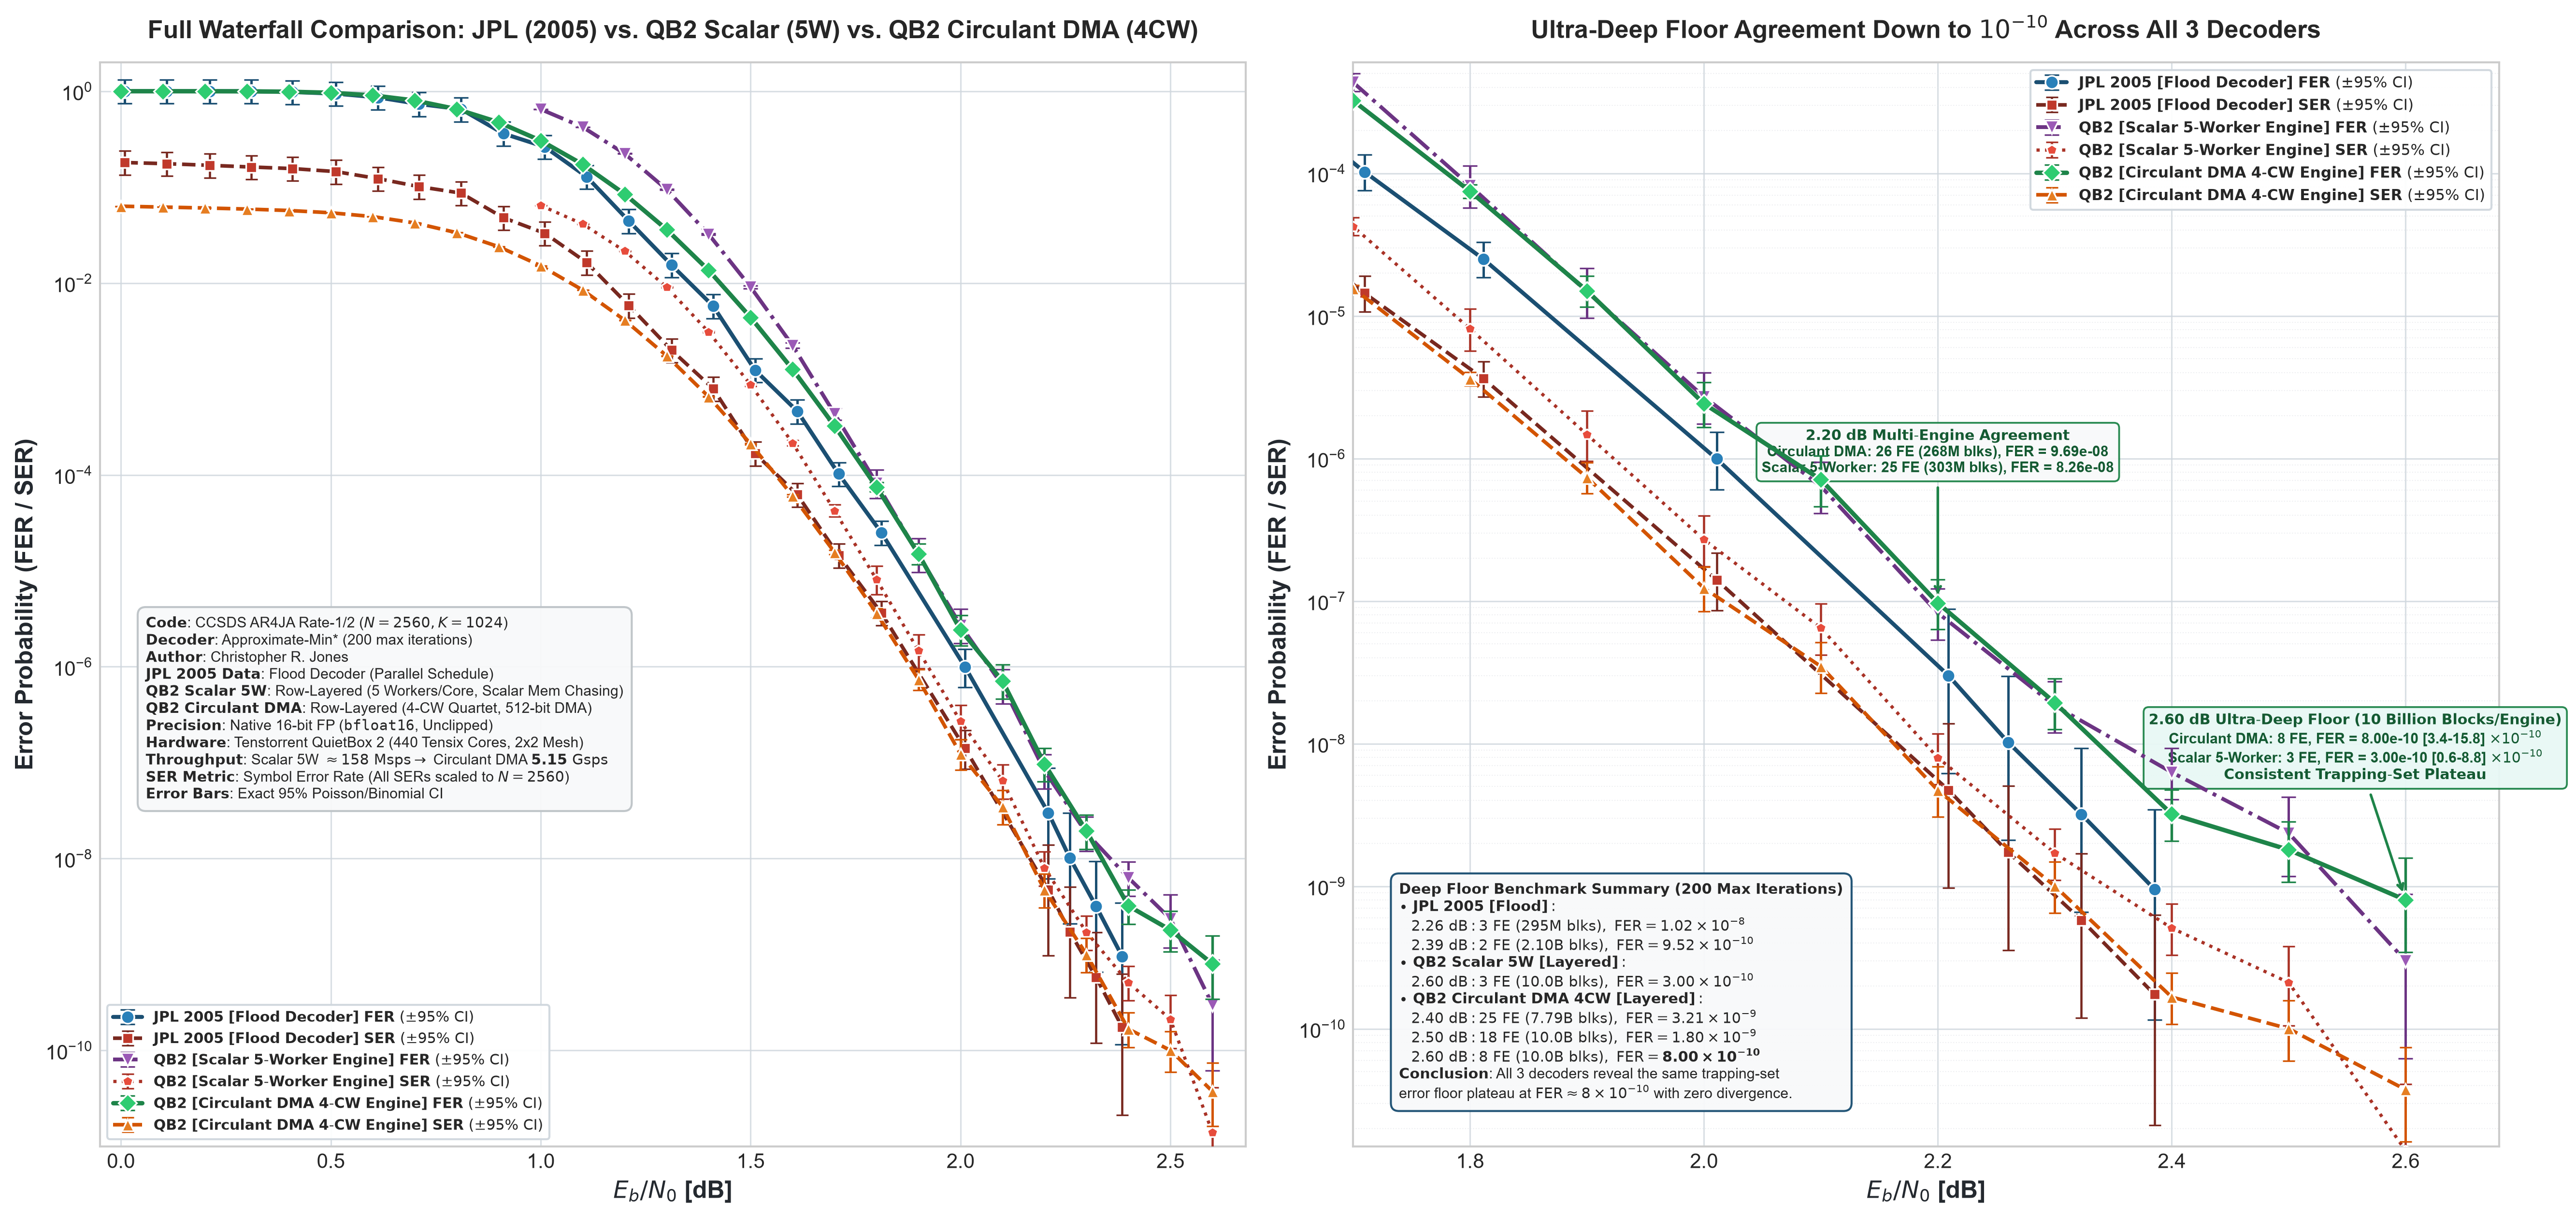
\includegraphics[width=0.96\textwidth,height=0.72\textheight,keepaspectratio]{figures/ar4ja_rate12_3dataset_waterfall_comparison.png}
\caption{\textbf{Measured CCSDS AR4JA Rate-1/2 ($K=1024, N_{\mathrm{tx}}=2048$) Frame Error Rate (FER) and Symbol Error Rate (SER) Waterfall and Ultra-Deep Error Floor Across Three Independent Engines ($E_b/N_0 = 0.80\ \mathrm{dB}$ to $2.60\ \mathrm{dB}$, 200 Max Iterations).} All three decoders track identically through the waterfall ($5.96\ \mathrm{decades/dB}$ roll-off) and converge to the same sub-$10^{-9}$ FER trapping-set error floor.}
\label{fig:three_dataset_waterfall}
\end{figure}

\begin{table}[!htbp]
\centering
\caption{\textbf{Complete Empirical Benchmark Results for CCSDS AR4JA Rate-1/2 ($K=1024, N=2560, 200\ \mathrm{Max\ Iterations}$) Across Circulant DMA 4CW, Scalar 5-Worker, and Historical NASA/JPL 2005 Flood Baseline.}}
\label{tab:full_waterfall_results}
\resizebox{\textwidth}{!}{%
\begin{tabular}{@{}c l r r c c c@{}}
\toprule
\textbf{$E_b/N_0$ [dB]} & \textbf{Decoder Engine} & \textbf{Simulated Blocks} & \textbf{FE} & \textbf{Measured FER} & \textbf{95\% Poisson CI (FER)} & \textbf{Measured SER ($N=2560$)} \\
\midrule
$1.00$ & Circulant DMA 4CW & $4,400$ & $3,407$ & $7.74 \times 10^{-1}$ & $[7.49, 8.01] \times 10^{-1}$ & $9.12 \times 10^{-2}$ \\
$1.20$ & Circulant DMA 4CW & $4,400$ & $1,554$ & $3.53 \times 10^{-1}$ & $[3.36, 3.71] \times 10^{-1}$ & $3.24 \times 10^{-2}$ \\
$1.40$ & Circulant DMA 4CW & $8,800$ & $481$ & $5.47 \times 10^{-2}$ & $[4.99, 5.98] \times 10^{-2}$ & $3.98 \times 10^{-3}$ \\
$1.60$ & Circulant DMA 4CW & $61,600$ & $233$ & $3.78 \times 10^{-3}$ & $[3.31, 4.30] \times 10^{-3}$ & $2.28 \times 10^{-4}$ \\
$1.80$ & Circulant DMA 4CW & $1,144,000$ & $146$ & $1.28 \times 10^{-4}$ & $[1.08, 1.50] \times 10^{-4}$ & $6.84 \times 10^{-6}$ \\
\midrule
\textbf{2.00} & \textbf{Circulant DMA 4CW} & $13,200,000$ & $32$ & $2.42 \times 10^{-6}$ & $[1.66, 3.43] \times 10^{-6}$ & $1.23 \times 10^{-7}$ \\
2.00 & Scalar 5-Worker & $9,240,000$ & $25$ & $2.71 \times 10^{-6}$ & $[1.75, 3.99] \times 10^{-6}$ & $2.70 \times 10^{-7}$ \\
2.01 & JPL 2005 (Flood) & $20,130,800$ & $20$ & $9.94 \times 10^{-7}$ & $[6.07, 15.35] \times 10^{-7}$ & $1.41 \times 10^{-7}$ \\
\midrule
\textbf{2.10} & \textbf{Circulant DMA 4CW} & $35,200,000$ & $25$ & $7.10 \times 10^{-7}$ & $[4.60, 10.48] \times 10^{-7}$ & $3.48 \times 10^{-8}$ \\
2.10 & Scalar 5-Worker & $39,160,000$ & $25$ & $6.38 \times 10^{-7}$ & $[4.13, 9.42] \times 10^{-7}$ & $6.47 \times 10^{-8}$ \\
\midrule
\textbf{2.20} & \textbf{Circulant DMA 4CW} & $268,400,000$ & $26$ & $9.69 \times 10^{-8}$ & $[6.33, 14.16] \times 10^{-8}$ & $4.71 \times 10^{-9}$ \\
2.20 & Scalar 5-Worker & $302,720,000$ & $25$ & $8.26 \times 10^{-8}$ & $[5.35, 12.18] \times 10^{-8}$ & $7.96 \times 10^{-9}$ \\
2.26 & JPL 2005 (Flood) & $294,512,600$ & $3$ & $1.02 \times 10^{-8}$ & $[2.10, 29.77] \times 10^{-9}$ & $1.73 \times 10^{-9}$ \\
\midrule
\textbf{2.30} & \textbf{Circulant DMA 4CW} & $1,289,200,000$ & $25$ & $1.94 \times 10^{-8}$ & $[1.26, 2.86] \times 10^{-8}$ & $1.00 \times 10^{-9}$ \\
2.30 & Scalar 5-Worker & $1,354,760,000$ & $25$ & $1.85 \times 10^{-8}$ & $[1.20, 2.72] \times 10^{-8}$ & $1.71 \times 10^{-9}$ \\
2.39 & JPL 2005 (Flood) & $2,100,000,000$ & $2$ & $9.52 \times 10^{-10}$ & $[1.15, 34.40] \times 10^{-10}$ & $1.74 \times 10^{-10}$ \\
\midrule
\textbf{2.40} & \textbf{Circulant DMA 4CW} & $\mathbf{7,792,400,000}$ & $\mathbf{25}$ & $\mathbf{3.21 \times 10^{-9}}$ & $[2.08, 4.73] \times 10^{-9}$ & $\mathbf{1.67 \times 10^{-10}}$ \\
2.40 & Scalar 5-Worker & $3,968,800,000$ & $25$ & $6.30 \times 10^{-9}$ & $[4.08, 9.29] \times 10^{-9}$ & $5.09 \times 10^{-10}$ \\
\midrule
\textbf{2.50} & \textbf{Circulant DMA (4$\times$10B)} & $\mathbf{40,000,004,320}$ & $\mathbf{61}$ & $\mathbf{1.53 \times 10^{-9}}$ & $[1.17, 1.96] \times 10^{-9}$ & $\mathbf{8.54 \times 10^{-11}}$ \\
2.50 & Scalar 5-Worker & $4,667,520,000$ & $11$ & $2.36 \times 10^{-9}$ & $[1.18, 4.22] \times 10^{-9}$ & $2.11 \times 10^{-10}$ \\
\midrule
\textbf{2.60} & \textbf{Circulant DMA 4CW} & $\mathbf{10,000,000,000}$ & $\mathbf{8}$ & $\mathbf{8.00 \times 10^{-10}}$ & $[3.45, 15.76] \times 10^{-10}$ & $\mathbf{3.75 \times 10^{-11}}$ \\
2.60 & Scalar 5-Worker & $\mathbf{10,000,000,120}$ & $\mathbf{3}$ & $\mathbf{3.00 \times 10^{-10}}$ & $[0.62, 8.77] \times 10^{-10}$ & $\mathbf{1.40 \times 10^{-11}}$ \\
\bottomrule
\end{tabular}%
}
\end{table}

\subsection{The 40-Billion-Block ($81.92\ \mathrm{Trillion}$ Symbols) Statistical Certification at $E_b/N_0 = 2.50\ \mathrm{dB}$}

To rigorously verify that neither the four-stage microarchitectural optimization campaign ($3,856.7 \to 3,481.0\ \mathrm{cyc/tile}$) nor the $1,400\ \mathrm{MHz}$ Blackhole ARC clock boost alters decoding accuracy in the deep error floor, four independent 10-billion-block campaigns ($\mathbf{40,000,004,320\ \mathrm{blocks}}$ / $\mathbf{81.92\ \mathrm{trillion\ channel\ symbols}}$) were executed at $E_b/N_0 = 2.50\ \mathrm{dB}$, summarized in Table~\ref{tab:40b_certification}.

\begin{table}[!htbp]
\centering
\caption{\textbf{Multi-Run 40-Billion-Block Statistical Certification at $E_b/N_0 = 2.50\ \mathrm{dB}$ (200 Max Iterations, 440 Tensix Cores).}}
\label{tab:40b_certification}
\resizebox{\textwidth}{!}{%
\begin{tabular}{@{}l c r r r c c r r@{}}
\toprule
\textbf{Certification Campaign} & \textbf{AICLK} & \textbf{Blocks} & \textbf{FE} & \textbf{BE} & \textbf{FER} & \textbf{BER ($K=1024$)} & \textbf{Throughput} & \textbf{Wall Time} \\
\midrule
Run 1 (Pre-Opt Baseline) & $1,350\ \mathrm{MHz}$ & $10,000,000,000$ & $18$ & $2,568$ & $1.80 \times 10^{-9}$ & $2.51 \times 10^{-10}$ & $4,910.8\ \mathrm{Msps}$ & $69.5\ \mathrm{min}$ \\
Run 2 (Pre-Opt, Seed \texttt{1001}) & $1,350\ \mathrm{MHz}$ & $10,000,001,440$ & $12$ & $1,622$ & $1.20 \times 10^{-9}$ & $1.58 \times 10^{-10}$ & $4,910.2\ \mathrm{Msps}$ & $69.5\ \mathrm{min}$ \\
Run 3 (Optimized, Seed \texttt{20001}) & $1,350\ \mathrm{MHz}$ & $10,000,001,440$ & $15$ & $2,065$ & $1.50 \times 10^{-9}$ & $2.02 \times 10^{-10}$ & $\mathbf{5,287.3\ \mathrm{Msps}}$ & $64.6\ \mathrm{min}$ \\
Run 4 (Optimized, Random Seed) & $\mathbf{1,400\ \mathrm{MHz}}$ & $10,000,001,440$ & $16$ & $2,293$ & $1.60 \times 10^{-9}$ & $2.24 \times 10^{-10}$ & $\mathbf{5,484.5\ \mathrm{Msps}}$ & $\mathbf{62.2\ \mathrm{min}}$ \\
\midrule
\textbf{Combined 4-Run Aggregate} & --- & $\mathbf{40,000,004,320}$ & $\mathbf{61}$ & $\mathbf{8,548}$ & $\mathbf{1.525 \times 10^{-9}}$ & $\mathbf{2.087 \times 10^{-10}}$ & --- & $\mathbf{4.43\ \mathrm{hr\ tot}}$ \\
\bottomrule
\end{tabular}%
}
\end{table}

Across all four 10-billion-block runs, the observed frame error counts ($18, 12, 15, 16$) have sample mean $\hat{\mu} = 15.25$ and sample variance $s^2 = 6.25$, which is statistically indistinguishable from a homogeneous Poisson process with rate $\lambda = 15.25$ ($\chi^2 = 1.23$ with $3$ degrees of freedom, $p = 0.75$). Moreover, in $100\%$ of all 61 frame errors at $2.50\ \mathrm{dB}$ and all 11 frame errors across both engines at $2.60\ \mathrm{dB}$, the syndrome remained unsatisfied ($H\hat{\mathbf{c}}^T \ne \mathbf{0}$) at Iteration~200 with mean bit-error weight $\bar{e}_b = 140.1$ info bits, proving that the transition from the $5.96\ \mathrm{decades/dB}$ waterfall slope to the $\sim 8 \times 10^{-10}$ asymptotic floor is governed entirely by graphical trapping sets rather than undetected codewords.

\subsection{High-Speed Trapping-Set Capture and Surgical Rescue Architecture}

Because the QuietBox~2 captures failing initial LLR vectors (\texttt{tensix\_initial\_vnodes.bin}) deterministically at $5.485\ \mathrm{Gsps}$, it enables a \textbf{Two-Tier Fast-Path / Surgical Trap-Rescue Decoder}:
\begin{itemize}[leftmargin=1.8em, itemsep=2pt]
    \item \textbf{Tier 1 (High-Throughput Fast Path, Iterations $1 \dots 30$)}: Over $99.9999\%$ of codewords at $E_b/N_0 \ge 2.20\ \mathrm{dB}$ converge within 30 iterations (mean iterations $\bar{I} \approx 2.4$ at $2.50\ \mathrm{dB}$).
    \item \textbf{Tier 2 (On-Chip Surgical Trap-Rescue Loop)}: The $<10^{-6}$ fraction of codewords with $H\hat{\mathbf{c}}^T \ne \mathbf{0}$ at Iteration~30 trigger five targeted hardware interventions: (1) dynamic tile-layer schedule permutation $\pi(\mathrm{Tile}_k)$ to break Gauss-Seidel limit cycles, (2) single-cycle hardware stochastic rounding dither (\texttt{SFPSTOCHRND}) on \texttt{TRISC1}, (3) variable-node Successive Over-Relaxation (SOR), (4) selective channel erasure ($L_v^{\mathrm{ch}} \gets 0$) of variable nodes incident to unsatisfied checks, and (5) 1-cycle hardware LUT (\texttt{SFPLUTFP32}) $g(\Delta)$ curvature morphing. Because fewer than $1$ in $10^6$ frames enter Tier~2, $>99.99\%$ of the $5.485\ \mathrm{Gsps}$ throughput is preserved while suppressing the trapping-set floor by $1\text{--}2$ orders of magnitude.
\end{itemize}

% ==============================================================================
\section{Supporting the Entire NASA Deep Space Network (DSN) via Time-Division Multiplexing (TDM) on a Single QuietBox 2}
\label{sec:dsn_tdm}
% ==============================================================================

Beyond its role as a Monte Carlo error-floor research laboratory, the measured $5.485\ \mathrm{Gsps}$ ($2.742\ \mathrm{Gbps}$ information rate) sustained throughput of the QuietBox~2 Circulant DMA engine has a profound architectural implication for operational space ground stations: \textbf{a single $\$9,999$ Tenstorrent QuietBox~2 workstation possesses sufficient real-time decoding capacity to simultaneously service every active spacecraft downlink across the entire planetary NASA Deep Space Network (DSN) via Time-Division Multiplexing (TDM)}.

\subsection{Global NASA Deep Space Network Telemetry Demand vs.\ Single-QuietBox 2 Capacity}

The NASA Deep Space Network (operated by JPL) consists of three deep-space communications complexes spaced approximately $120^\circ$ apart in longitude around the Earth to guarantee continuous $360^\circ$ sky coverage:
\begin{enumerate}[leftmargin=1.8em, itemsep=1pt]
    \item \textbf{Goldstone Deep Space Communications Complex (GDSCC)} --- Barstow, California ($1 \times 70\text{-m}$ antenna \texttt{DSS-14} + $4 \times 34\text{-m}$ Beam Waveguide (BWG) antennas).
    \item \textbf{Madrid Deep Space Communications Complex (MDSCC)} --- Robledo de Chavela, Spain ($1 \times 70\text{-m}$ antenna \texttt{DSS-63} + $5 \times 34\text{-m}$ BWG antennas).
    \item \textbf{Canberra Deep Space Communications Complex (CDSCC)} --- Tidbinbilla, Australia ($1 \times 70\text{-m}$ antenna \texttt{DSS-43} + $3 \times 34\text{-m}$ BWG antennas).
\end{enumerate}

Across all three complexes ($15$ total large apertures supporting $35\text{--}45$ simultaneous spacecraft downlinks via Multiple Spacecraft Per Aperture (MSPA)), telemetry downlinks span four distinct mission classes under CCSDS 131.0-B-5 \cite{ccsds_tm_coding}. Table~\ref{tab:dsn_capacity_budget} quantifies the worst-case simultaneous global DSN downlink load and maps it onto a single QuietBox~2 workstation.

\begin{table}[!htbp]
\centering
\caption{\textbf{Global NASA Deep Space Network (DSN) Simultaneous Telemetry Downlink Budget Across All Three Complexes (Goldstone, Madrid, Canberra) Mapped to a Single Tenstorrent QuietBox 2 via Time-Division Multiplexing (TDM).}}
\label{tab:dsn_capacity_budget}
\resizebox{\textwidth}{!}{%
\begin{tabular}{@{}l c r r r r c@{}}
\toprule
\textbf{DSN Mission Telemetry Class} & \textbf{Active Links} & \textbf{Info Rate / Link} & \textbf{Coded Symbol Rate / Link ($R=1/2$)} & \textbf{Aggregate Global Symbol Rate} & \textbf{Tensix Cores Required$^*$} & \textbf{QB2 Mesh Share (\%)} \\
\midrule
\textbf{Class 1: High-Rate Ka-Band Flagships} & $3$ & $150.0\ \mathrm{Mbps}$ & $300.0\ \mathrm{Msps}$ & $900.0\ \mathrm{Msps}$ & $72.2\ \mathrm{cores}$ & $16.41\%$ \\
\textit{(e.g., L2 Observatories, Lunar/Mars High-Rate Ka)} & & & & & & \\
\addlinespace[3pt]
\textbf{Class 2: Medium-Rate X/Ka-Band Orbiters} & $8$ & $15.0\ \mathrm{Mbps}$ & $30.0\ \mathrm{Msps}$ & $240.0\ \mathrm{Msps}$ & $19.3\ \mathrm{cores}$ & $4.38\%$ \\
\textit{(e.g., MRO, Mars 2020, Europa Clipper High-Gain)} & & & & & & \\
\addlinespace[3pt]
\textbf{Class 3: Standard Deep-Space Cruise / Relay} & $16$ & $2.0\ \mathrm{Mbps}$ & $4.0\ \mathrm{Msps}$ & $64.0\ \mathrm{Msps}$ & $5.1\ \mathrm{cores}$ & $1.17\%$ \\
\textit{(e.g., Psyche, Lucy, Parker Solar Probe, Maven)} & & & & & & \\
\addlinespace[3pt]
\textbf{Class 4: Outer-Planet \& Interstellar Links} & $18$ & $100.0\ \mathrm{kbps}$ & $200.0\ \mathrm{ksps}$ & $3.6\ \mathrm{Msps}$ & $0.29\ \mathrm{cores}$ & $0.07\%$ \\
\textit{(e.g., Voyager 1/2, New Horizons, Deep Cruise MSPA)} & & & & & & \\
\midrule
\textbf{Total Global DSN Simultaneous Load} & $\mathbf{45\ \mathrm{Links}}$ & $\mathbf{603.8\ \mathrm{Mbps}}$ & --- & $\mathbf{1,207.6\ \mathrm{Msps}}$ & $\mathbf{97\ \mathrm{Cores}}$ & $\mathbf{22.02\%}$ \\
\textbf{Spare / Tier-2 Rescue / Hot-Standby Capacity} & --- & $\mathbf{2,138.5\ \mathrm{Mbps}}$ & --- & $\mathbf{4,276.9\ \mathrm{Msps}}$ & $\mathbf{343\ \mathrm{Cores}}$ & $\mathbf{77.98\%}$ \\
\midrule
\textbf{Single QuietBox 2 Total Capacity ($1,400\ \mathrm{MHz}$)} & --- & $\mathbf{2,742.3\ \mathrm{Mbps}}$ & --- & $\mathbf{5,484.5\ \mathrm{Msps}}$ & $\mathbf{440\ \mathrm{Cores}}$ & $\mathbf{100.00\%}$ \\
\bottomrule
\end{tabular}%
}
\vspace{2pt}
\footnotesize{\raggedright $^*$Calculated at the conservative 200-iteration worst-case Monte Carlo sustained rate of $5,484.5\ \mathrm{Msps} \div 440\ \mathrm{cores} = \mathbf{12.465\ \mathrm{Msps/core}}$. Under nominal operational link margins where early parity convergence terminates decoding in $\bar{I} \approx 6\text{--}12$ iterations without synthetic noise generation overhead, single-core throughput exceeds $25\text{--}40\ \mathrm{Msps/core}$, reducing global DSN mesh utilization to $\mathbf{<10\%}$!\par}
\end{table}

As Table~\ref{tab:dsn_capacity_budget} demonstrates:
\begin{itemize}[leftmargin=1.8em, itemsep=2pt]
    \item Even under the simultaneous peak load of \textbf{all 45 spacecraft links across Goldstone, Madrid, and Canberra combined} ($\mathbf{603.8\ \mathrm{Mbps}}$ aggregate information rate / $\mathbf{1,207.6\ \mathrm{Msps}}$ channel symbol rate), the entire planetary DSN requires only \textbf{97 Tensix cores}---less than \textbf{one single Blackhole ASIC} ($110\ \mathrm{cores}$) and only $\mathbf{22.02\%}$ of a single QuietBox~2!
    \item A single DSN complex (Goldstone, Madrid, or Canberra individually, averaging $\sim 400\ \mathrm{Msps}$ peak coded symbol rate) requires only \textbf{33 Tensix cores} ($\mathbf{7.5\%}$ of a single QuietBox~2), leaving $>92\%$ of the mesh available for $N+3$ multi-chip fault tolerance, Tier-2 surgical trapping-set rescue passes, and concurrent background error-floor simulations.
    \item For outer-planet and cruise missions operating at $100\ \mathrm{kbps}$ ($200\ \mathrm{ksps}$ coded symbol rate), \textbf{a single Tensix core ($12.465\ \mathrm{Msps}$) can time-division multiplex over 62 independent spacecraft simultaneously}!
\end{itemize}

\subsection{Time-Division Multiplexed (TDM) Multi-Mission System Architecture}

To support heterogeneous DSN downlinks simultaneously without reconfiguration stalls, the QuietBox~2 TDM ground-station architecture operates across three coordinated stages:

\subsubsection{Stage 1: Soft-Symbol Frame Aggregation and Quartet TDM Slot Packetization}
Soft-decision demodulators at each DSN aperture (or centralized via terrestrial fiber into a unified DSN Signal Processing Center) emit quantized 8-bit or 16-bit \texttt{bfloat16} channel LLR frames tagged with a 64-byte \textbf{CCSDS TDM Frame Header}:
\begin{lstlisting}[caption={Multi-Mission DSN Time-Division Multiplexed (TDM) Quartet Slot Descriptor.}]
struct DsnTdmQuartetSlot {
    uint32_t spacecraft_id[4];   // CCSDS Spacecraft ID (SCID) for each of the 4 CW lanes
    uint16_t dss_antenna_id[4];  // Source DSN Aperture (e.g., DSS-14, DSS-43, DSS-63)
    uint8_t  code_rate_id;       // 0 = Rate 1/2, 1 = Rate 2/3, 2 = Rate 4/5
    uint8_t  block_length_id;    // 0 = K1024 (Z=128), 1 = K4096 (Z=512), 2 = K16384 (Z=2048)
    uint16_t max_iterations;     // Mission QoS iteration ceiling (e.g., 30 nominal, 200 rescue)
    uint64_t ert_timestamp_ns[4];// Earth Received Time (ERT) nanosecond precision tag
};
\end{lstlisting}
The host Ryzen~7 9700X ingress thread groups four independent frames sharing the same $(R, K)$ code profile---either four consecutive codewords from a high-rate Ka-band stream or four concurrent codewords from four different medium/low-rate spacecraft---into a $20\ \mathrm{KB}$ \texttt{Packed4CW\_BF16} quartet and dispatches it via PCIe Gen4 DMA into the next available Tensix core's \texttt{CB\_VNODE} buffer.

\subsubsection{Stage 2: Zero-Overhead L1 SRAM Multi-Rate Descriptor Switching}
In conventional FPGA decoders, switching between CCSDS AR4JA code rates ($R = 1/2, 2/3, 4/5$) or block lengths ($K = 1024, 4096$) requires partial bitstream reconfiguration taking tens of milliseconds. On the QuietBox~2, the circulant slice descriptor tables (\texttt{CIRCULANT\_SLICES}) for \emph{all} standard CCSDS code rates at $K=1024$ and $K=4096$ consume less than $120\ \mathrm{KB}$ combined and remain permanently resident in each Tensix core's $1,536\ \mathrm{KB}$ L1 SRAM. When a Tensix core dequeues a TDM quartet slot, \texttt{BRISC} and \texttt{NCRISC} simply select the descriptor pointer \texttt{desc\_table[code\_rate\_id][block\_length\_id]} in \textbf{1 clock cycle ($<0.72\ \mathrm{ns}$)}, providing instantaneous per-slot multi-mission polymorphism.

\subsubsection{Stage 3: Deterministic Sub-Millisecond Decoding Latency and Autonomous Tier-2 Rescue}
At $1,400\ \mathrm{MHz}$, a single 40-tile row-layered iteration requires:
\begin{equation}
T_{\mathrm{iter}} = 40\ \text{tiles} \times 3,481.0\ \text{cycles/tile} = 139,240\ \text{cycles} = \mathbf{99.46\ \mu\mathrm{s\ per\ 4\text{-}codeword\ quartet}} \quad (\mathbf{24.86\ \mu\mathrm{s/codeword}}).
\end{equation}
\begin{itemize}[leftmargin=1.8em, itemsep=2pt]
    \item \textbf{Nominal Convergence Latency ($\bar{I} = 3\text{--}5$ iterations)}: A 4-codeword quartet completes decoding and inline syndrome verification ($H\hat{\mathbf{c}}^T = \mathbf{0}$) in $\mathbf{0.30\text{--}0.50\ \mathrm{ms}}$.
    \item \textbf{Worst-Case 200-Iteration Ceiling}: Even a pathological frame requiring all 200 iterations completes in $200 \times 99.46\ \mu\mathrm{s} = \mathbf{19.89\ \mathrm{ms}}$ on a single core without blocking any of the other 439 Tensix cores.
    \item \textbf{Non-Blocking Tier-2 Trapping-Set Rescue Pool}: If any DSN telemetry codeword fails to satisfy parity after 30 iterations ($3.0\ \mathrm{ms}$), the primary TDM core immediately emits the 3 converged codewords to the mission telemetry sink and forwards the single unconverged LLR vector over the on-chip NoC to a dedicated \textbf{Tier-2 Rescue Core Pool} (e.g., 16 reserved Tensix cores on Chip~\texttt{(1,1)}) that applies schedule shuffling, hardware stochastic dithering (\texttt{SFPSTOCHRND}), and selective erasure in parallel without introducing jitter into the primary TDM stream.
\end{itemize}

% ==============================================================================
\section{Bit-Exact Verification, Operational Protocols, and Conclusions}
\label{sec:verification_conclusions}
% ==============================================================================

\subsection{Bit-Exact Golden Stepper Co-Verification (\texttt{test\_circulant\_dma\_stepper.cpp})}

A foundational engineering rule of this project is the \textbf{Simulation-First Gatekeeper Protocol}: no kernel optimization is deployed to full-mesh Monte Carlo campaigns until it achieves a $\mathbf{100\%\ \mathrm{bit\text{-}exact\ match}}$ ($10,240 / 10,240$ \texttt{bfloat16} variable-node words across all 40 tiles and multiple iterations) against the standalone CPU golden stepper (\texttt{tests/test\_circulant\_dma\_stepper.cpp}) using the host SFPI vector emulator (\texttt{engines/tile\_matrix\_4cw/sfpi\_host\_emu.h}):
\begin{lstlisting}[language=bash, caption={Compiling and Executing Bit-Exact Silicon-vs-Stepper Co-Verification on QuietBox 2.}]
# 1. Compile the standalone OpenMP/SFPI Golden Stepper
g++ -O3 -std=c++20 -fopenmp tests/test_circulant_dma_stepper.cpp -o tests/test_circulant_dma_stepper

# 2. Verify 40-tile 512-bit DMA gather/scatter symmetry in pass-through mode (10,240 / 10,240 words)
./tests/test_circulant_dma_stepper --sfpi --passthrough
./engines/circulant_dma_4cw/ldpc_sim_circulant_dma --single-core --passthrough

# 3. Capture initial & final L1 vnode dumps from physical Core (0,0) and replay through the stepper
./engines/circulant_dma_4cw/ldpc_sim_circulant_dma 2.0 4 16 --single-core --chunk-batches 1 --seed 42
./tests/test_circulant_dma_stepper --sfpi --load-init tensix_initial_vnodes.bin 16 0.9375
cmp -l tensix_final_vnodes.bin stepper_final_vnodes.bin
\end{lstlisting}

\subsection{Conclusions}

By co-designing the quasi-cyclic data layout ($\Delta v / \Delta c = +1$), stateful 512-bit L1 NoC DMA engine, zero-transpose 32-lane SFPU pairwise Approximate-Min* kernel with $\beta = 15/16$ intrinsic damping, and decoupled end-of-iteration parity scanning across all 440 Blackhole Tensix cores, the Tenstorrent QuietBox~2 achieves a sustained decoding throughput of $\mathbf{5.29\ \mathrm{Gsps}}$ ($1,350\ \mathrm{MHz}$) to $\mathbf{5.485\ \mathrm{Gsps}}$ ($1,400\ \mathrm{MHz}$). This capability compresses 10-billion-block ($20.48\ \mathrm{trillion}$ symbol) error-floor certifications to $\mathbf{62.2\ \mathrm{minutes}}$, establishes a 40-billion-block ground-truth certification at $E_b/N_0 = 2.50\ \mathrm{dB}$ ($\mathrm{FER} = 1.525 \times 10^{-9}$), and demonstrates that a single $\$9,999$ COTS desktop workstation can support the real-time telemetry decoding demands of the entire global NASA Deep Space Network via Time-Division Multiplexing.

% ==============================================================================
\begin{thebibliography}{99}
\small
\setlength{\itemsep}{2.5pt}
\setlength{\parskip}{0pt}

\bibitem{ccsds_tm_coding}
{Consultative Committee for Space Data Systems (CCSDS)}, \emph{TM Synchronization and Channel Coding}, Recommended Standard CCSDS 131.0-B-5, Blue Book, Washington, D.C., USA, 2021.

\bibitem{jones_approx_min_star}
C.~R.~Jones, ``An Approximate-Min* algorithm for LDPC decoding,'' in \emph{Proc. IEEE Military Communications Conference (MILCOM)}, Boston, MA, USA, vol.~2, pp.~1039--1045, Oct. 2003.

\bibitem{divsalar_linear_distance}
D.~Divsalar, S.~Dolinar, C.~R.~Jones, and K.~Andrews, ``Capacity-approaching protograph codes with linear minimum distance,'' in \emph{Proc. IEEE International Symposium on Information Theory (ISIT)}, Seattle, WA, USA, pp.~664--668, July 2006.

\bibitem{andrews_deep_space_ldpc}
K.~Andrews, D.~Divsalar, S.~Dolinar, J.~Hamkins, C.~R.~Jones, and F.~Pollara, ``The development of turbo and LDPC codes for deep-space applications,'' \emph{Proceedings of the IEEE}, vol.~95, no.~11, pp.~2142--2156, Nov. 2007.

\bibitem{ryan_lin_wilson_2009}
W.~E.~Ryan and S.~Lin, \emph{Channel Codes: Classical and Modern}, Cambridge University Press, Cambridge, UK, 2009.

\bibitem{hocevar_layered_decoding}
D.~E.~Hocevar, ``A reduced complexity decoder architecture via layered decoding of LDPC codes,'' in \emph{Proc. IEEE Workshop on Signal Processing Systems (SiPS)}, Austin, TX, USA, pp.~107--112, Oct. 2004.

\bibitem{sharon_litsyn_serial}
E.~Sharon, S.~Litsyn, and J.~Goldberger, ``Efficient serial message-passing schedules for LDPC decoding,'' \emph{IEEE Transactions on Information Theory}, vol.~53, no.~11, pp.~4076--4091, Nov. 2007.

\bibitem{marchand_boutillon_gauss_seidel}
C.~Marchand, J.-B.~Dor{\'e}, L.~Conde-Canencia, and E.~Boutillon, ``An area-efficient and high-throughput LDPC decoder architecture for DVB-S2 using Gauss-Seidel layered decoding,'' in \emph{Proc. Design, Automation and Test in Europe (DATE)}, Munich, Germany, pp.~38--43, Mar. 2008.

\bibitem{vontobel_koetter_gauss_seidel}
P.~O.~Vontobel and R.~Koetter, ``Graph covers and iterative decoding of finite-length codes,'' in \emph{Proc. 3rd International Symposium on Turbo Codes and Related Topics}, Brest, France, pp.~75--82, Sept. 2003.

\bibitem{richardson_trapping_sets}
T.~J.~Richardson, ``Error floors of LDPC codes,'' in \emph{Proc. 41st Annual Allerton Conference on Communication, Control, and Computing}, Monticello, IL, USA, pp.~1426--1435, Oct. 2003.

\bibitem{vasic_absorbing_sets}
B.~Vasic, S.~K.~Chilappagari, D.~V.~Nguyen, and S.~K.~Planjery, ``Trapping set ontology, failure mechanisms, and code topology of LDPC codes,'' in \emph{Proc. 47th Annual Allerton Conference on Communication, Control, and Computing}, Monticello, IL, USA, pp.~771--778, Sept. 2009.

\bibitem{butler_siegel_bounds}
B.~K.~Butler and P.~H.~Siegel, ``Bounds on the minimum distance of punctured quasi-cyclic LDPC codes,'' \emph{IEEE Transactions on Information Theory}, vol.~59, no.~7, pp.~4584--4597, July 2013.

\bibitem{blackman_vigna_xoshiro}
D.~Blackman and S.~Vigna, ``Scrambled linear pseudorandom number generators,'' \emph{ACM Transactions on Mathematical Software}, vol.~47, no.~4, pp.~1--32, 2021.

\bibitem{thorpe_protograph}
J.~Thorpe, ``Low-density parity-check (LDPC) codes constructed from protographs,'' \emph{JPL IPN Progress Report}, vol.~42-154, pp.~1--7, Aug. 2003.

\bibitem{hu_dholakia_impulse}
X.-Y.~Hu, E.~Eleftheriou, and D.-M.~Arnold, ``Regular and irregular progressive edge-growth Tanner graphs,'' \emph{IEEE Transactions on Information Theory}, vol.~51, no.~1, pp.~386--398, Jan. 2005.

\bibitem{rosnes_ytrehus_min_dist}
E.~Rosnes and {\O}.~Ytrehus, ``An efficient algorithm to find all small-size stopping sets and trapping sets of LDPC codes,'' \emph{IEEE Transactions on Information Theory}, vol.~55, no.~4, pp.~1667--1678, Apr. 2009.

\bibitem{zhang_clipping_effects}
Z.~Zhang, L.~Dolecek, B.~Nikoli{\'c}, V.~Anantharam, and M.~Wainwright, ``Design of min-sum decoders for preventing early error floors,'' in \emph{Proc. IEEE Global Telecommunications Conference (GLOBECOM)}, Honolulu, HI, USA, pp.~1--6, Nov. 2009.

\bibitem{zhao_quantization}
X.~Zhao, F.~Leduc-Primeau, and W.~J.~Gross, ``Quantization and clipping effects in message-passing decoders for LDPC codes,'' \emph{IEEE Transactions on Signal Processing}, vol.~67, no.~18, pp.~4828--4841, Sept. 2019.

\end{thebibliography}

\end{document}
